\documentclass[11pt]{article}
\usepackage[margin=1in]{geometry}
\usepackage{graphicx}
\usepackage{float}
\usepackage[section]{placeins}
\renewcommand{\topfraction}{0.9}
\renewcommand{\bottomfraction}{0.9}
\renewcommand{\textfraction}{0.08}
\renewcommand{\floatpagefraction}{0.95}
\setcounter{topnumber}{3}
\setcounter{bottomnumber}{2}
\setcounter{totalnumber}{6}
\usepackage{booktabs}
\usepackage{xcolor}
\usepackage{amsmath}
\usepackage{lmodern}
\usepackage{authblk}
\usepackage{multicol}
\usepackage{url}
\usepackage[hidelinks]{hyperref}
\setlength{\parindent}{0pt}
\setlength{\parskip}{5pt}
\graphicspath{{figures/}}

\newcounter{fignum}
\newcounter{tabnum}
\newcommand{\fig}[3]{%
  \begin{figure}[!htbp]\centering
  \includegraphics[width=\linewidth]{#1}\par\vspace{2pt}
  \refstepcounter{fignum}\label{#2}%
  {\small\raggedright\textbf{Figure \thefignum.} #3\par\vspace{1pt}
  \footnotesize\textit{Sources:} Zillow Research (ZHVI and ZORI) and the U.S. Census Bureau (ACS estimates and Census geography), as applicable.\par}
  \end{figure}}
\newcommand{\figH}[3]{%
  \begin{figure}[H]\centering
  \includegraphics[width=\linewidth]{#1}\par\vspace{2pt}
  \refstepcounter{fignum}\label{#2}%
  {\small\raggedright\textbf{Figure \thefignum.} #3\par\vspace{1pt}
  \footnotesize\textit{Sources:} Zillow Research (ZHVI and ZORI) and the U.S. Census Bureau (ACS estimates and Census geography), as applicable.\par}
  \end{figure}}
\newcommand{\tab}[3]{%
  \begin{table}[!htbp]\centering
  \refstepcounter{tabnum}\label{#2}%
  {\small\raggedright\textbf{Table \thetabnum.} #3\par}\vspace{3pt}
  \input{tables/#1}
  \end{table}}
\newcommand{\tabH}[3]{%
  \begin{table}[H]\centering
  \refstepcounter{tabnum}\label{#2}%
  {\small\raggedright\textbf{Table \thetabnum.} #3\par}\vspace{3pt}
  \input{tables/#1}
  \end{table}}
\title{Rough Draft:\\Remote Work and Urban Housing Prices in Eight Sun Belt Metros}
\author[1]{Sai Krishna Varshith Danda}
\author[1]{Gayathri Kota}
\author[1]{Eshitha Chowdary Kaka}
\author[1]{Zain Khan}
\affil[1]{Arizona State University, Tempe, AZ 85281, USA}
\date{November 21, 2026}

\begin{document}
\maketitle

\begin{abstract}
The COVID-19 shift to remote and hybrid work may have weakened the value of living near a central business district. We test
whether the within-metropolitan house-price gradient flattened after 2020 and remained flatter through 2025 in Atlanta, Austin,
Charlotte, Dallas, Las Vegas, Nashville, Phoenix, and Tampa. We combine monthly Zillow home values and rents with Census
geography and pre-pandemic American Community Survey characteristics for 1,082 ZIP codes. Exploratory comparisons, a ZIP
fixed-effects event study with spatial block-bootstrap intervals, clustering, and leave-one-metro-out prediction models give a
consistent but qualified result. The pooled gradient moved outward after 2019, but Atlanta drives much of the late-period result
and metro patterns differ sharply. Pooled across the eight metros, a ZIP code 10 miles farther from the center gained about 1.15
percent more between December 2019 and December 2025, but that point estimate falls to about 0.09 percent when Atlanta is excluded. A
ZIP code's pre-pandemic work-from-home share does not have a stable relationship with later
growth once income, housing, prior growth, and spatial dependence are considered. Price paths form a continuum more than distinct
groups, and predictive models explain only 10-30 percent of growth variation in a metro they have not seen. The evidence is
consistent with a persistent spatial revaluation in selected metros, not a uniform Sun Belt Donut Effect and not a causal estimate
of remote work.
\end{abstract}

\section{Introduction}

Where people live depends partly on where they work. In the monocentric city model, households accept higher housing costs near
the center in exchange for shorter commutes \cite{alonso1964location}. Remote work lowers the number of commutes and should
therefore weaken that central-location premium. Before 2020, working from home was too uncommon to test this prediction at housing-
market scale. The pandemic created a sudden test: households and real-estate demand moved away from dense centers, producing what
Ramani and Bloom called the ``Donut Effect'' \cite{ramani2021donut}, while price and rent gradients flattened in many U.S. metros
\cite{gupta2022flattening}.

The unsettled question is persistence. Remote work remained above its pre-pandemic level even as return-to-office policies spread,
and recent work finds that the Donut Effect persisted where hybrid work remained common \cite{barrero2023evolution,ramani2024reshapes}.
At the same time, rising mortgage rates, mortgage lock-in, changing amenities, and new housing supply complicate any claim that
remote work caused later price patterns \cite{howard2023short,fonseca2024mortgage}. Most within-metro evidence also emphasizes
large, dense cities and ends before the 2023-2025 return-to-office period.

We study eight fast-growing Sun Belt metros: Atlanta, Austin, Charlotte, Dallas, Las
Vegas, Nashville, Phoenix, and Tampa. These places are useful tests because many grew around automobiles and multiple job centers.
Distance from one downtown may always have
been a weak summary of location value, leaving less of a central premium for remote work to erase. Phoenix, for example, has
multiple employment centers with different industry mixes \cite{leslie2010identification}; Dallas-Fort Worth is explicitly
multinodal \cite{waddell1993residential}.

The project asks three questions:
\begin{enumerate}
\item How did the relationship between distance from the center and ZIP-level housing-price growth change from 2018 through 2025?\par
\item Did ZIP codes with more pre-pandemic work-from-home exposure grow differently after 2020 than otherwise comparable ZIP codes?\par
\item What price-path groups emerge from 2018-2025, and what characteristics distinguish them?\par
\end{enumerate}
We expected the price gradient to flatten in 2020-2022 and remain flatter through 2025; a positive relationship between
pre-pandemic work-from-home share and later growth; and three to five recognizable price-path groups. The analysis supports the
first expectation only in selected metros, finds no consistent support for the second, and shows that the third describes convenient
slices of a continuum rather than naturally separated groups.

\subsection*{Key Terms and Measures}

Five definitions make the analysis easier to follow. \textbf{Home value} means Zillow's estimate of the typical mid-tier home in a
ZIP code, not the median price of only the homes sold that month. \textbf{Distance} means miles from the ZIP's geographic center to
the nearer named city hall in the formal models. The exploratory plots use the first-named city hall so they can show how the
answer changes when a second center is introduced in Dallas-Fort Worth and Tampa-St. Petersburg. Either version is a reproducible
measure of centrality, not a claim that every resident works downtown.
\textbf{Gradient} means the estimated relationship between housing value or growth and that distance. A negative level gradient
means homes tend to be less expensive farther out. A positive growth gradient means outer ZIP codes appreciated faster during the
period. \textbf{Flattening} means that the central price advantage weakened; it does not necessarily mean outer homes became more
expensive than central homes. Finally, \textbf{work-from-home exposure} means the share of workers reporting that they usually
worked from home in the 2015-2019 ACS, before the housing changes studied here.

Most reported gradient coefficients use a 10-mile distance increment. For example, a 2025 event-study coefficient of $+$1.15
means that, pooled across the eight metros, a ZIP 10 miles farther out gained about 1.15 percent more from December 2019
to December 2025 than an otherwise equivalent nearer ZIP in the same metro. It does not mean that the outer ZIP grew 1.15 percent
per year or that remote work caused the difference. Exposure coefficients are reported per five percentage points of baseline
work-from-home share. Growth slopes in the exploratory period comparisons are annualized, while event-study coefficients are
cumulative changes relative to December 2019.

\begin{table}[!tbp]\centering
\refstepcounter{tabnum}\label{tab:rqsummary}
{\small\raggedright\textbf{Table \thetabnum.} Research questions, hypotheses, primary tests, and final interpretations. This table
is a guide to the argument; the estimates and uncertainty intervals appear in the Results section.\par}\vspace{4pt}
{\small\setlength{\tabcolsep}{3pt}\renewcommand{\arraystretch}{1.18}
\begin{tabular}{@{}p{.14\linewidth}p{.22\linewidth}p{.25\linewidth}p{.32\linewidth}@{}}
\toprule
Question & Original expectation & Primary evidence & Final interpretation \\
\midrule
SQ1: distance gradient & Sharp flattening in 2020-2022 that persists through 2025 & Period slopes, maps, ZIP fixed-effects event
study, spatial block bootstrap, rent and two-center checks & Partial support. The pooled gradient moves outward by 2025, but
Atlanta drives the clearest persistent result; other metros show delay, reversal, pre-trends, or little change. \\
SQ2: remote-work exposure & Higher pre-2020 work-from-home share predicts stronger post-2020 growth & Nested exposure
regressions, county mixed model, spatial intervals, Moran's $I$, feature ablation and permutation importance & Not supported
consistently. The coefficient changes sign with controls, and exposure adds almost no held-out predictive value. \\
SQ3: price-path groups & Three to five distinct trajectories separated more by exposure and housing than by distance & Monthly
indexed paths, principal components, $k$-means, Ward clustering, Gaussian mixture, silhouette width and method agreement & Paths
are meaningfully different but weakly separated. Four groups summarize a continuum; they are not stable natural types. \\
\bottomrule
\end{tabular}}
\end{table}

We keep the three questions separate because they make different claims. A change in the distance gradient is a claim about
\emph{where} housing demand shifted within a metro. A relationship between work-from-home exposure and growth is a claim about
\emph{which neighborhood characteristics} accompany that shift. A set of price-path clusters is a claim about \emph{how many
distinct trajectories} appear in the data. None of those claims automatically proves the others. Outer ZIP codes can appreciate
without being populated by remote workers, a high-work-from-home ZIP code can be close to downtown, and a clustering algorithm can
create groups even when the underlying paths form a continuum. Keeping the questions separate prevents a descriptive Donut Effect
from being treated as direct evidence of a remote-work mechanism.

The paper makes four contributions. First, it extends the observation window through December 2025, covering both the early
pandemic and the later period of hybrid work, higher interest rates, and return-to-office policies. Second, it concentrates on
eight Sun Belt metros in which polycentric form makes the standard downtown-distance measure a demanding test. Third, it treats
spatial dependence as part of the design by using block-bootstrap intervals and geographic cross-validation rather than adding a
generic caveat after estimation. Fourth, it reports negative and unstable results alongside positive ones. The goal is not to
force one national story onto every metro, but to determine where the proposed story fits and where it does not.

The paper is organized from theory to evidence. Section 2 reviews the urban-economics argument, pandemic evidence,
and the gap concerning persistence in Sun Belt metros. Section 3 describes the linked Zillow, Census, and geographic data and the
decisions required to make ZIP-level comparisons credible. Section 4 presents the exploratory analysis. Section 5 explains the
event study, exposure models, clustering analysis, and validation design, and Section 6 reports their results. Sections 7 through
9 discuss the findings, ethical considerations, limitations, and future research before Section 10 concludes.

\section{Prior Research}

\subsection{From the monocentric model to remote work}

Urban theory predicts that commuting costs are capitalized into housing prices. Telecommuting should allow households to move
farther from work while reducing total commute travel, although residential location can also influence who chooses to telecommute
\cite{mokhtarian2004telecommuting}. That reverse-causality problem remains central: people may move because they can work remotely,
or high-growth places may attract remote workers after prices begin rising.

The pandemic evidence shows a large spatial revaluation. Ramani and Bloom documented households and businesses moving from city
centers toward suburbs \cite{ramani2021donut}. Gupta and coauthors found that rent gradients went from clearly negative to nearly
flat in many metros and that price gradients moved in the same direction \cite{gupta2022flattening}. Brueckner, Kahn, and Lin
formalized the mechanism as a new work-from-home spatial equilibrium \cite{brueckner2023spatial}. Evidence across OECD countries
also shows demand spreading toward lower-density and more affordable places \cite{ahrend2023expanding}.

The classical monocentric model begins with a tradeoff between land and commuting. Land is cheaper farther from the center, but a
longer commute consumes time and money. In equilibrium, housing prices or rents compensate households for the higher commuting
cost. A reduction in the number of commute days lowers the effective cost of distance and should flatten the price gradient. This
prediction is intuitive, but its empirical meaning depends on the city. If employment is already dispersed among several centers,
distance from city hall may not approximate commuting cost. A flatter estimated gradient can also arise because central prices
fall, outer prices rise, or both. The same slope can therefore represent different market processes.

Telecommuting research before 2020 anticipated both the location response and the identification problem. Workers who telecommute
may choose homes farther from work because they commute less often, but workers with unusually long commutes may also be the most
likely to request remote arrangements \cite{mokhtarian2004telecommuting}. The direction of causality is difficult to establish even
with individual workers and becomes harder with neighborhood averages. This is why the present study uses a pre-2020 exposure
measure and why it does not interpret a post-2020 correlation as a treatment effect.

\subsection{The pandemic revaluation of urban space}

The speed and scale of the 2020 shock made the spatial mechanism visible in a way earlier telecommuting could not. Offices closed,
urban amenities were restricted, households sought more space, mortgage rates fell, and fiscal support raised purchasing power.
Several of these shocks favored suburban housing at the same time. Change-of-address data showed movement away from dense central
areas, while housing indexes showed relative gains at greater distances from downtown. The label ``Donut Effect'' usefully
describes the geography, but it does not by itself identify which pandemic mechanism produced it.

Prices and rents also answer different questions. A house price reflects the expected future stream of housing services and is
sensitive to mortgage rates and investor expectations. Rent more directly measures the current price of occupying a unit and does
not depend on a tenant's mortgage financing. Gupta and coauthors found stronger early flattening in rents than in house prices,
while prices initially appeared to anticipate some return of central demand \cite{gupta2022flattening}. Comparing the two outcomes
after 2022 is therefore informative even though Zillow's rent coverage is much smaller.

The effect is unlikely to be uniform across neighborhoods or metros. The ability to work remotely differs by occupation, income,
and industry; housing supply differs by regulation and available land; and the value of proximity differs with transit, congestion,
and the location of employment centers. National averages can consequently conceal places that flatten, reverse, or show no
pre-pandemic gradient to begin with. This heterogeneity motivates the metro-specific estimates reported below.

\subsection{Persistence, return to office, and competing explanations}

Cause and persistence are less certain. Dingel and Neiman's occupation-based measure estimates which jobs can be done at home
rather than who moved after 2020 \cite{dingel2020jobs}. Mondragon and Wieland similarly use pre-pandemic remote-work exposure and
find a large national housing-demand effect \cite{mondragon2022housing}. Later evidence finds persistent decentralization through
2023 and 2024 \cite{ramani2024reshapes}, but housing-supply responses may reduce the long-run price effect
\cite{howard2023short}. Mortgage lock-in also reduced mobility after rates rose, limiting households' ability to undo pandemic-era
moves \cite{fonseca2024mortgage}.

Persistence is not equivalent to proof of a permanent preference change. A gradient can remain flatter because hybrid work makes
distance less costly, because homeowners are locked into low mortgage rates and do not move, because new construction is
concentrated in outer areas, or because central amenities recover slowly. Return-to-office mandates can also affect households
unevenly: a worker commuting two days per week may still value a different location than a worker commuting five. The period from
2023 through 2025 is therefore best treated as a new market regime rather than a simple reversal period.

The timing creates an empirical advantage and a complication. If the gradient changed only during 2020-2022 and then returned to
its earlier level, temporary pandemic conditions would be a plausible explanation. If it remained changed through 2025, lasting
hybrid work would be consistent with the evidence. Yet mortgage rates rose sharply at almost the same time that offices reopened.
Metro-by-year fixed effects absorb shocks shared by all ZIP codes in a metro, but they cannot remove a rate shock that affects
central and outer neighborhoods differently. The rent comparison and the post-2022 coefficient path are checks on this problem,
not complete solutions.

\subsection{Why the Sun Belt is a distinct test}

Many Sun Belt metros developed during the automobile era and spread across large areas with weak transit orientation. Their
municipal boundaries, downtowns, and employment centers often do not coincide. In Dallas-Fort Worth, two large central cities and
many suburban employment concentrations make a single radial measure especially restrictive. Tampa-St. Petersburg presents a
similar two-center problem across the bay. Phoenix and Las Vegas contain large areas in which topography, master-planned
development, and the location of newer housing can generate nonlinear price-distance relationships.

These features do not make distance irrelevant. They change what a distance coefficient means. A negative pre-pandemic level
gradient would show a downtown premium despite dispersed development; a near-zero gradient could mean no premium or offsetting
submarkets; and a positive gradient could reflect high-value suburban corridors rather than a pandemic relocation. The project
therefore retains the conventional city-hall measure for comparability with earlier studies but supplements it with maps, smooth
curves, directional patterns, quality flags, and two-center robustness checks.

\subsection{Research gap and analytical strategy}

This project contributes a ZIP-level view through 2025 in metros whose polycentric form makes a one-center model especially
contestable. It combines descriptive spatial evidence with an event study, explicit spatial resampling, path clustering, and
out-of-metro validation. Because distance is continuous and the pandemic affected every location, the event-study coefficients
require stronger assumptions than a conventional treated-versus-untreated design \cite{callaway2024did}. We therefore interpret
them as descriptive changes consistent or inconsistent with a remote-work mechanism, not as causal effects.

Earlier studies establish the plausibility of decentralization and provide national or large-city estimates. The remaining gap is
not whether Sun Belt metros appeared somewhere in those samples. It is whether their within-metro gradients remained changed
during the overlapping return-to-office and high-rate years, whether pre-pandemic exposure explains differences among their ZIP
codes, and whether neighborhood paths separate into types that a single slope misses. Addressing all three questions in the same
sample also reveals when apparently supportive results fail to reinforce one another. For example, a positive pooled gradient can
coexist with negligible predictive importance for work-from-home share. That distinction becomes central in the results.

To answer those questions on a common basis, we assemble one ZIP-level analytical system that links housing outcomes, baseline
neighborhood characteristics, and geography. The following section explains what each source measures, why it is appropriate for
the research questions, how the samples are constructed, and which limitations enter before any model is estimated.

\section{Data and Preparation}

\subsection{Sources and sample}

The primary outcome is Zillow's ZIP-level, all-homes, mid-tier Zillow Home Value Index (ZHVI), a smoothed and seasonally adjusted
estimate of typical home value \cite{zillow2026data}. The secondary outcome is the Zillow Observed Rent Index (ZORI). ZORI provides
a useful check because rent does not respond directly to mortgage financing, although its coverage is much thinner. Neighborhood
characteristics come from the 2015-2019 and 2019-2023 American Community Survey 5-year estimates, including work-from-home share,
occupation, household income, population, and housing structure \cite{census2026acs}. Census ZCTA boundaries and Gazetteer
centroids provide geography.

ZHVI is preferable to a raw median sale price because it is designed to follow the value of a typical home even when the mix of
properties sold changes. That advantage comes with two limitations. The index is model-based rather than a direct average of
transactions, and smoothing can mute sudden changes. We use the all-homes, mid-tier series so the same concept is available across
metros and months. Values are nominal. This choice keeps the interpretation close to what households observed in local markets,
but a common inflation shock is not removed from descriptive growth rates. Metro-by-time effects remove common nominal changes
within the formal event study.

ZORI uses advertised rents and requires enough listings to produce a stable index. Its thinner coverage is not random: outer and
lower-density ZIP codes are less likely to have a complete rental series. Rent results consequently describe a more central and
urban subset than the price results. We hold the rent sample fixed across periods so changes in the estimated gradient do not arise
from ZIP codes entering or leaving the panel. The comparison is treated as a robustness exercise rather than a second outcome with
equal evidentiary weight.

The ACS baseline release combines surveys collected from 2015 through 2019. Its work-from-home share therefore predates the
pandemic, avoiding the most direct form of reverse causality in which remote workers move into a ZIP after its prices rise. The
same release supplies household income, population, occupation, and housing-stock controls. Five-year estimates improve coverage
for small geographies but average conditions over time and carry sampling error. We flag a work-from-home estimate as unreliable
when its margin of error exceeds half of the estimate and preserve that flag for sensitivity checks.

The balanced house-price sample contains 1,082 ZIP codes with the required December values from 2017 through 2025. The event study
uses that sample. Exposure and prediction models use 1,073 complete cases; clustering uses the 1,072 ZIP codes observed in all 96
months from January 2018 through December 2025. The balanced rent comparison contains 478 ZIP codes and primarily represents the
inner and middle parts of each metro.

The analysis begins from the metro names attached to Zillow's ZIP-level series. We standardize ZIP identifiers as five-character
strings and retain the eight named metropolitan areas. Census variables are reported for ZIP Code Tabulation Areas (ZCTAs), which
approximate but do not exactly reproduce postal ZIP codes. The join therefore requires an explicit audit. Twelve Zillow ZIP codes
are present in the housing data but not the preferred crosswalk and are retained with a flag; five crosswalk-only ZIP codes have no
housing series and cannot enter the outcome panel. Reporting these mismatches avoids presenting a geographic join as exact.

The December-balanced sample supports comparisons across annual endpoints without allowing changing coverage to alter the result.
Clustering requires the stricter 96-month balanced panel because distance-based algorithms cannot compare paths with arbitrary
gaps. Only ten ZIP codes are lost between the annual and monthly definitions. The exposure sample loses nine ZIP codes because of
missing ACS controls, leaving 1,073 observations in 82 counties. These small differences explain why sample sizes change across
tables; they do not reflect discretionary deletion of inconvenient observations.

\tab{t_coverage}{tab:coverage}{Coverage after the source files are joined. The analysis retains ZIP codes with complete observations
for the outcome and period required by each method rather than silently treating missing values as zeros.}

\figH{2_1a_distributions}{fig:distributions}{Distributions of the main housing, geographic, and neighborhood variables used in the
analysis. Skewed variables motivate logarithmic transformations, while the metro panels show why pooled summaries are not treated
as representative of every local market.}

\FloatBarrier

\subsection{Geography, outcomes, and quality checks}

Distance is the great-circle distance from each ZCTA centroid to a named city hall. The event study, exposure models, and prediction
models use distance to the nearer named city hall, which matters only in Dallas-Fort Worth and Tampa-St. Petersburg. The exploratory
slopes begin with the first-named city hall and then show the nearer-center version as a robustness check. We compute annualized growth for 2018-2019, 2020-2022, and
2023-2025, and index monthly paths to December 2019. Work-from-home exposure is measured with the 2015-2019 ACS release so the
measure predates the price changes it is intended to explain.

City hall is a reproducible center and matches a common convention in the literature, but it is not assumed to be the unique job
center. Coordinates were checked against public building locations, and distances were recomputed from both Gazetteer centroids
and ZCTA polygon centroids as a consistency check. For Dallas-Fort Worth and Tampa-St. Petersburg, the primary two-center measure
is distance to the nearer city hall. We also inspect each side separately because replacing two distances with their minimum can
hide differences in the price levels of the two cores.

Growth is calculated from the index endpoints and annualized so periods of different lengths can be compared on the same scale.
The 2018-2019 period establishes the immediate pre-pandemic pattern, 2020-2022 captures the rapid pandemic appreciation and the
beginning of monetary tightening, and 2023-2025 covers the later adjustment. Monthly values are retained even when the main table
uses December endpoints. Price paths are normalized to December 2019 for clustering so groups reflect subsequent relative changes
rather than the dollar level of homes.

The pipeline keeps all ZIP codes but records quality flags rather than silently discarding edge cases. Checks cover metro
crosswalk mismatches, implausible distances, missing months, ACS margins of error, and outer ZIP codes that are geographically
detached from the main cluster. This matters because several apparent gradients, especially Phoenix's, are sensitive to a small
number of distant ZIP codes. Every cleaned table is rebuilt by the numbered pipeline, and separate audit scripts recompute the
figures and all numerical claims used in the report.

The decision to flag rather than delete is substantive. Peripheral ZIP codes are precisely where the hypothesis predicts stronger
post-2020 growth, so a rule that automatically removes distant observations could remove the phenomenon of interest. Conversely,
an isolated ZIP may belong only administratively to the metro and exert high leverage on a linear slope. We therefore show full
and flag-free estimates and interpret a result that disappears without flagged ZIP codes as sensitive rather than selecting one
sample after seeing the sign.

\fig{2_1c_flags_by_distance}{fig:qualitydistance}{Data-quality flags by distance band. The columns progress from the closest ZIP
codes to the farthest and then show the full sample. Missing rent coverage and unreliable work-from-home estimates are concentrated
in the outer band, which is why the sensitivity analysis keeps distance and data quality separate.}

Initial distributions also shaped the transformations. Home values, income, and population are right-skewed, so models use logs
or within-metro relative versions where appropriate. Shares remain in percentage-point units for interpretability. Correlations
among work-from-home share, income, and initial home value are reported rather than hidden inside a multivariable model. The strong
overlap among these measures is one reason coefficient stability across nested specifications matters more than the nominal
significance of a single regression.

All source-specific cleaning is implemented before analysis. The housing files are reshaped from wide monthly columns into panels;
dates and identifiers are validated; ACS count variables are converted into shares using common denominators; geographic files are
projected only for mapping, while distances are calculated geodesically; and outputs are written as clean tables used by both
notebooks and reports. This separation prevents figures from applying undocumented filters that differ from the regression sample.

With the measurement choices and analytical samples fixed, we first examine the raw spatial patterns. This exploratory step shows
where a straight-line distance measure is useful, where it is misleading, and which patterns need a more formal test.

\section{Exploratory Data Analysis}

\subsection{What the raw patterns show}

For each metro and period, we compare price levels and annualized growth with distance using linear fits, smooth curves, distance
bands, and within-metro value groups. The level and growth relationships answer different questions. A negative level gradient
means central ZIP codes are more expensive at a point in time. A positive growth gradient means outer ZIP codes appreciated faster
during a period. A metro can therefore retain an expensive center while its outer areas catch up.

The expected flattening is not uniform across the eight metros. Atlanta is the clearest case: outer ZIP codes gained relative to
inner ZIP codes during 2020-2022 and continued gaining through 2025. Austin turns outward only in 2023-2025. Tampa flattens during
the pandemic period but reverses afterward when distance is measured from Tampa city hall. Charlotte, Dallas, and Las Vegas show little linear change. Phoenix moves in the
opposite direction in the full sample, but much of that result disappears when flagged outer ZIP codes are removed. Nashville's
outer advantage begins before 2020, which weakens a pandemic interpretation.

The maps and smooth fits explain why some linear slopes are unstable. Expensive ZIP codes form directional patches rather than
rings in several metros; Phoenix and Las Vegas have curved level relationships; and Dallas and Fort Worth sit at different price
levels. A single distance from city hall cannot fully represent those housing markets.

The distributions also separate the housing boom from the later adjustment. Every metro shows strong appreciation during
2020-2022, but the 2023-2025 period is much weaker and turns negative in several markets. That common slowdown is why the analysis
uses metro-by-year effects in the event study instead of treating every post-2022 decline as evidence about distance or remote work.

Level and growth gradients do not tell the same story. Atlanta, Austin, Charlotte, and Nashville still have expensive central areas
in 2025 even when some outer ZIP codes gained faster for part of the period. Dallas and Las Vegas have relatively flat average level
slopes, while Phoenix is better described by a curved surface. We therefore keep the level, growth, and time-path views together.

\figH{2_2_slope_summary}{fig:slopes}{Annualized growth-versus-distance slopes by metro and period. Metros are listed alphabetically,
followed by the two alternate-center checks. Positive values mean ZIP codes farther from the center appreciated faster. Comparing
the three periods separates a pre-existing pattern from a pandemic shift and a later reversal.}

Figure~\ref{fig:slopes} makes the cross-metro differences visible. Atlanta moves from a negative pre-2020 growth slope to positive
slopes in both later periods. Measured from Tampa city hall, Tampa has a positive 2020-2022 slope but a negative 2023-2025 slope,
which is a reversal rather than persistence. Nashville already has an outward growth pattern before 2020, so its later result cannot be read as a new pandemic
break. The remaining estimates are smaller, less stable, or sensitive to the choice of center.

\figH{2_3b_level_quintile_maps}{fig:valuemaps}{December 2019 home values grouped into fifths within each metro. Metro panels are in
alphabetical order. The maps show whether expensive ZIP codes form a ring around the center or a directional patch that a single
distance coefficient would average together.}

The maps make the limits of a single distance measure concrete. Atlanta and Charlotte have expensive areas extending in more than
one direction, while Austin and Nashville show broad corridors rather than complete rings. Dallas and Tampa contain two visible
centers, and the Phoenix pattern follows a long east-west urban footprint. These shapes explain why two ZIP codes at the same
distance can have very different home values and why the linear slope is treated as a summary, not a complete model of the market.

\figH{2_5b_relative_paths}{fig:paths}{Monthly home-value paths by distance band within each metro, expressed relative to that metro's
monthly median and indexed to December 2019. Metros are ordered alphabetically, and bands run from the lightest inner-ring line to
the darkest outer-ring line. Persistent separation after 2020 would indicate that outer ZIP codes gained relative to the rest of
their own metro.}

\subsection{How the exploratory analysis changed the design}

The exploratory work changed the formal analysis in four ways. First, the large differences across metros required metro-specific
estimates rather than one pooled line. Second, nearby ZIP codes moved together, so intervals that treat every ZIP code as independent
would be too narrow. Third, work-from-home share overlapped strongly with income and initial home value, which required nested
controls and a separate prediction test. Fourth, the first cluster solution had only modest separation, so we compare several
clustering methods instead of treating one set of groups as a discovered truth.

The maps also changed how we interpret distance. If high-value ZIP codes form a ring, distance is a reasonable summary. If they lie
mainly north, east, or along one development corridor, the same slope averages a directional pattern. We use the plots to diagnose
that problem, not to select the result we prefer.

These comparisons remain descriptive because they do not hold constant permanent ZIP differences or metro-wide annual shocks. The
next section explains the models used to test whether the gradient changed after 2019, whether work-from-home exposure adds a stable
signal, and whether the price paths form distinct groups.

\section{Methods}

\subsection{Analytical sequence and decision rules}

After constructing and validating the sample, we first used exploratory analysis to determine which spatial patterns required
formal testing. This stage was not a separate report placed in front of the models; it directly changed the final design. First,
linear gradients differed sharply across metros and were sometimes curved, so pooled results had to
be accompanied by metro estimates, smooth plots, and two-center checks. Second, neighboring ZIP codes moved together, making
independent-error intervals implausible. Third, work-from-home share was closely related to income and initial value, requiring
nested controls and explicit pre-trend adjustment. Fourth, the initial four-cluster solution had only modest silhouette width,
requiring comparison across algorithms rather than treating one partition as discovered truth.

This sequence matters for interpretation. The exploratory slopes summarize patterns in separate periods, while the event study
holds constant every time-invariant ZIP characteristic and every metro-wide annual shock. The exploratory exposure scatterplots
show raw association, while the later models ask whether that association remains after measured confounders and prior growth are
held fixed. The exploratory clusters provide a readable visualization, while the method comparison evaluates whether the data
actually contain separated groups. The final analysis therefore refines, and sometimes weakens, the initial conclusions rather
than duplicating them.

The analysis follows the research questions in a fixed order. Exploratory maps and slopes establish what the raw spatial patterns
look like and where a one-center summary may fail. The event study then tests whether the distance gradient changed relative to
2019 while holding constant permanent ZIP differences and metro-wide annual shocks. Exposure regressions and geographic
prediction evaluate whether baseline work-from-home share supplies a stable explanatory or transferable signal. Clustering asks a
different question about whether monthly price paths form distinct types, and it is evaluated only after the distance and exposure
results are established. Robustness checks finally test whether the conclusions depend on flagged ZIP codes, the choice of center,
or the use of ownership prices instead of rents.

We use the same interpretation rule throughout: a result receives substantive weight only when its direction, uncertainty, and
geographic pattern agree across reasonable specifications. Statistical significance in one specification is not treated as
sufficient when the sign changes with defensible controls, a spatial interval crosses zero, a pre-trend is present, or the result
does not transfer to a held-out metro. This rule explains both why several initial patterns are retained descriptively and why they
lead to qualified final conclusions.

\subsection{Event study of the price gradient}
\label{sec:event}

For ZIP code $z$ in metro $m$ and December of year $t$, we estimate
\begin{equation}
\ln V_{zt}=\alpha_z+\gamma_{m(z),t}+\sum_{k\ne2019}\beta_k
\left(\frac{D_z}{10}\right)\mathbf{1}[t=k]+\varepsilon_{zt},
\label{eq:event}
\end{equation}
where $V_{zt}$ is home value, $D_z$ is miles from the center, $\alpha_z$ is a ZIP fixed effect, and $\gamma_{m,t}$ is a
metro-by-year effect. Each $\beta_k$ is the additional percentage gain since December 2019 for a ZIP 10 miles farther from the
center. The 2017 and 2018 coefficients are pre-trend checks.

The ZIP fixed effect absorbs a ZIP's stable home quality, long-run desirability, and fixed distance. The metro-by-year effect
absorbs the average annual path of each metro, including metro-wide changes in employment, mortgage conditions, and population.
Identification comes from whether the cross-sectional distance gradient changes relative to 2019 within the same metro. The model
does not require outer ZIP codes to have the same starting value as inner ZIP codes. It does require the coefficient on distance to
be a meaningful average of the spatial change, which is why nonlinear and metro-specific evidence remains important.

The pre-period coefficients are not a formal proof of parallel trends because distance is continuous and only two pre-2019 years
are available. They are nevertheless an essential diagnostic. A large 2017 or 2018 coefficient means the gradient was already
moving before the pandemic, so a later coefficient cannot be attributed solely to the 2020 shock. We emphasize this issue for
Nashville and distinguish an acceleration of an existing trend from the beginning of a new one.

Ordinary intervals are inappropriate when nearby ZIP codes move together. We therefore divide each metro into spatial cells about
15 miles across, redraw whole cells with replacement within metro, and refit the model 1,000 times. Percentile block-bootstrap
intervals are the primary event-study intervals. The pooled model is accompanied by metro-specific estimates because a common
average can hide opposing patterns.

The grid contains 235 populated cells, with 16 to 44 in each metro. Resampling occurs within metro so every bootstrap draw retains
all eight metropolitan areas while allowing local spatial blocks to receive different weights. The procedure preserves more of
the dependence among nearby ZIP codes than row-level resampling. It is not a perfect model of spatial covariance: results can
depend on cell size and the number of metros is small. We therefore compare block and ordinary intervals and focus on conclusions
that are not artifacts of treating 1,082 ZIP codes as independent observations.

The event study answers where the price gradient changed, but it does not identify why it changed. We next test whether
pre-pandemic work-from-home exposure helps explain which ZIP codes grew faster within the same metropolitan market.

\subsection{Work-from-home exposure and spatial dependence}
\label{sec:exposure}

We regress annualized ZIP growth on 2015-2019 work-from-home share. The coefficient is reported for a five-point increase in that
share. The model includes metro fixed effects and controls for distance, income, December 2019 home value, detached-house share,
and the share of units in buildings with 20 or more units. A second specification adds pre-2020 growth. We compare robust OLS,
county-clustered OLS, a mixed model with a county random intercept, and OLS with the same spatial block bootstrap. Because the
exposure bootstrap is skewed, the primary reported interval is bias-corrected and accelerated (BCa), alongside percentile, basic,
and symmetric alternatives.

The nested specifications are intended to expose, rather than conceal, sensitivity. Metro fixed effects compare ZIP codes only
within the same housing market. Distance represents location; initial value and income represent neighborhood price and purchasing
power; housing structure captures differences between detached-home and large-building markets; and pre-2020 growth tests whether
post-2020 performance continues an earlier trajectory. If adding a defensible control reverses the exposure coefficient, the sign
is not interpreted as a stable substantive relationship even when one interval excludes zero.

County clustering and the mixed model address administrative nesting but not all spatial dependence. County boundaries can divide
nearby ZIP codes, and two distant ZIP codes within a large county need not share the same shock. The spatial bootstrap is therefore
the primary uncertainty procedure. The mixed model remains useful because it estimates how much residual variation lies between
counties, while the alternative interval constructions show how skew in the resampled coefficient distribution affects inference.

Moran's $I$ measures remaining spatial dependence using each ZIP's eight nearest neighbors and 999 random permutations. We
calculate it for metro-demeaned growth and for residuals from the controlled exposure model.

Moran's $I$ is positive when nearby observations are more similar than expected under random spatial arrangement. Testing both the
outcome and model residuals separates spatial pattern that measured covariates explain from pattern that remains unmodeled. The
eight-neighbor definition gives each ZIP the same number of links, avoiding the much larger neighbor counts that dense urban ZCTAs
would receive under a simple distance threshold.

The regression estimates show whether work-from-home exposure is associated with growth under specified controls. A separate
prediction exercise tests the stronger practical question: whether that exposure helps forecast an entirely unseen metropolitan
area rather than merely fitting spatial relationships already represented in the training sample.

\subsection{Prediction and validation}

Prediction models ask whether work-from-home share adds information about metro-relative growth after place, housing, income, and
prior growth are known. We compare ridge, lasso, random forest, and gradient boosting \cite{breiman2,sklearn}. Features enter in
nested sets: place and housing; then income and professional occupation share; then work-from-home share; then pre-2020 growth.
All preprocessing and tuning occur inside cross-validation.

Random train/test splits would place neighboring ZIP codes on both sides and overstate generalization. The primary evaluation
holds out one entire metro, trains on the other seven, and repeats eight times \cite{roberts}. Random five-fold scores are shown
only to quantify the optimism created by a geographically mixed split.

Hyperparameters are selected within each seven-metro training set using grouped inner folds. This nesting prevents the held-out
metro from influencing feature scaling, penalty strength, tree depth, or any other tuning decision. Performance is measured with
root mean squared error, mean absolute error, and out-of-sample $R^2$ relative to the training-set mean. A negative $R^2$ therefore
means that the model transfers worse than a constant prediction; a modest positive value indicates some portable information but
not accurate forecasting of individual ZIP codes.

Feature contribution is evaluated three ways. Nested feature sets show whether predictive performance improves when work-from-home
share is added. Lasso coefficients indicate whether a sparse linear model removes it. Permutation importance measures how much
held-out error rises when one feature is shuffled. None of these quantities is a causal effect. Their role is to test whether a
flexible predictive system finds a stable remote-work signal that the regression specification may have missed.

Exposure regressions and prediction complete the tests associated with the second research question. We then turn from explaining
growth with a predefined exposure to the third research question: whether the full monthly price histories themselves separate
into a small number of coherent trajectory types.

\subsection{Price-path clustering}

For each of 1,072 complete ZIP paths, we set December 2019 to 100, take logs, and compare $k$-means, Ward hierarchical clustering,
and a Gaussian mixture model. The mixture is fit to the first five principal components, which contain 98 percent of path
variation. Silhouette width evaluates separation, the adjusted Rand index evaluates agreement between methods, and BIC provides a
second diagnostic for the mixture model \cite{rousseeuw}.

The algorithms embody different ideas of a group. $k$-means searches for compact sets around average paths; Ward clustering builds
a hierarchy by merging paths that increase within-group variation least; and the Gaussian mixture allows probabilistic groups with
different covariance structures. Agreement between methods would suggest that a common structure is present beyond one
algorithm's assumptions. Low agreement, low silhouette width, or a BIC curve without a clear minimum suggests that any chosen
number of clusters is primarily a descriptive convenience.

Normalizing each path removes its pre-pandemic dollar level but does not remove differences in post-2019 amplitude. Principal
components reveal whether variation comes mainly from the size of appreciation, the timing of the peak, or the size of the later
correction. This diagnostic is important because four clusters that merely divide a single amplitude dimension should not be
described as four qualitatively different neighborhood histories.

\subsection{Reproducibility and analytical workflow}

The repository contains a numbered data pipeline, two executable notebooks, saved model outputs, figure and table builders, and
automated numerical checks. Source-specific cleaning occurs before analysis, and the EDA and formal models use the same cleaned
files. Figures and tables are generated from saved analytical outputs rather than manually re-entered values. This arrangement
creates an auditable chain from raw source, to cleaned panel, to model result, to the number or graphic shown in the paper.
The complete code appendix, notebooks, source files, and numerical audit scripts are available in the team repository at
\url{https://github.com/ZainKhanGit/Capstone-DAT490}. A file-level reproduction guide is provided in
\texttt{CODE\_APPENDIX.md}.

Before submission, the complete pipeline, report-table builders, both notebooks, and both numerical audit scripts are rerun in
sequence. The purpose is not only computational convenience. A single reproducible state prevents a revised model from appearing
in a table while an older estimate remains in the narrative or a figure. It also makes each sample restriction, transformation,
and quality flag traceable to a specific step in the workflow.

\section{Results}

The EDA identified the patterns that require formal testing. The results now follow the three research questions: first the event
study of the distance gradient, then the exposure and prediction tests, and finally the price-path groups. Robustness checks come
last so the main estimates and their limits can be read together.

\subsection{Event-study estimates}

Pooled across metros, the gradient coefficient is $+$0.48 percent per 10 miles in 2022, with a block interval from
$-$0.35 to $+$1.17. By 2025 it is $+$1.15, with an interval from $+$0.07 to $+$1.98. The 2022-2025 change is $+$0.67, with an
interval from $+$0.12 to $+$1.22. The pooled result therefore suggests that the outward revaluation persisted and widened after
2022, but it is not evidence of a common effect across metros.

Atlanta rises from $+$1.89 in 2022 to $+$4.98 in 2025, with its 2025 interval entirely above zero. Tampa's 2022 coefficient is
$+$1.51 and its 2025 coefficient is $+$1.73; the formal event study therefore shows no Tampa decline. Phoenix falls to $-$1.38 in
2025, while Charlotte, Dallas, and Las Vegas finish near zero. Nashville changes by $+$2.12 from 2022 to 2025, with an interval from
$+$1.26 to $+$2.74. That change is clearly positive, but Nashville's 2017 and 2018 coefficients are also nonzero, so it looks more
like a return to an earlier outward trend than a clean pandemic break. Spatial intervals are 1.1 to 3.0 times as wide as ordinary
intervals; several apparently precise OLS findings disappear once nearby ZIP codes are allowed to move together.

The pre-period checks are not clean for every specification. The pooled 2018 coefficient is $-$0.44 with an interval from $-$0.68
to $-$0.15. Nashville's 2017 and 2018 intervals exclude zero, as do Phoenix's. Charlotte's 2017 interval narrowly excludes zero.
These results do not invalidate the descriptive event study, but they rule out reading every post-2019 coefficient as a causal
effect of the pandemic or remote work.

\tabH{t_m_event_pre}{tab:eventpre}{Event-study coefficients for the pre-period and early post-period years. Every point estimate is
shown with its spatial block-bootstrap interval so the pre-trend assessment can be checked directly.}

\tabH{t_m_event_post}{tab:event}{Event-study coefficients for 2022 and 2025 and their change. The pooled estimate excluding Atlanta
is an algebraic point estimate from the saved metro weights; it has no bootstrap interval because the model was not resampled after
Atlanta was removed. All other intervals come from the spatial block bootstrap.}

The change between 2022 and 2025 is as important as either endpoint. A coefficient that rises after 2022 suggests continued
relative gains farther out; a stable coefficient suggests persistence without further widening; and a decline suggests partial
reversal. The pooled change of $+$0.67 is above zero under the main block interval, meaning the average gradient continued to move
outward rather than merely holding its 2022 position. Atlanta supplies the clearest metro-level version of that pattern. Nashville
also has a clearly positive 2022-2025 change, but its pre-trend makes the timing harder to attribute. Tampa changes by only $+$0.22,
with an interval from $-$1.25 to $+$1.33, so the formal result is persistence without detectable further widening or reversal.

Alternative interval constructions do not overturn the central event-study conclusion, although they affect borderline metros.
The pooled 2025 coefficient, the pooled 2022-2025 change, and Atlanta's 2025 coefficient remain above zero under basic and
symmetric intervals derived from the same resamples. Nashville's 2025 endpoint and Tampa's 2025 endpoint cross zero, even though
Nashville's change from 2022 is clearly positive. This distinction prevents an endpoint interval from being confused with an
interval for the change.

\fig{m_1_event_study}{fig:event}{Event-study coefficients relative to December 2019. A point is the additional percentage gain for
a ZIP code 10 miles farther out. Blue bands are 95\% spatial block-bootstrap intervals; orange dashes are ordinary intervals. The
pooled panel appears first, followed by the eight metros in alphabetical order.}

The event study strengthens the EDA in two ways. ZIP fixed effects show that the result is not simply produced by outer ZIP codes
having different permanent price levels, and metro-by-year effects show that it is not simply produced by one metro appreciating
faster than another. At the same time, the formal model confirms the EDA's warning about heterogeneity. A pooled coefficient is not
the effect experienced by a representative metro, because no single metro reproduces the pooled trajectory exactly.

The leave-Atlanta calculation makes that influence concrete. Applying the saved pooled-model weights to the seven remaining metro
coefficients gives about $+$0.09 in both 2022 and 2025, compared with $+$0.48 and $+$1.15 in the eight-metro model. This is a point
estimate only, not a new inferential result, because the spatial bootstrap was not rerun after excluding Atlanta.

\tabH{t_m_weights}{tab:eventweights}{Metro weights in the pooled event-study coefficient. Metros are listed alphabetically. The
weights sum to one and show that the pooled estimate reflects both the number of ZIP codes and the spread of distance within each
metro; it is not a simple average of eight metro coefficients.}

The formal estimates support a selective outward revaluation rather than a common Sun Belt effect. Distance shows where the change
occurred, but it does not explain the mechanism. The next analysis therefore asks whether pre-pandemic work-from-home exposure helps
explain which ZIP codes grew faster.

\subsection{Work-from-home exposure}

The exposure coefficient changes sign when controls are added. Without controls, the within-metro slope is $-$0.30 percentage
points of annual growth in 2020-2022 and $+$0.40 in 2023-2025 per five points of work-from-home share. With income, home value,
housing type, and distance held fixed, plain OLS gives $+$0.29 and $-$0.35; adding pre-2020 growth changes these to $+$0.26 and
$-$0.32. A sign that reverses with reasonable controls is not a stable remote-work result.

The BCa spatial intervals exclude zero in the controlled specifications, but the 2020-2022 conclusion changes under symmetric
and basic intervals, and the 2023-2025 basic interval just includes zero. The mixed model also produces a smaller late-period
coefficient. We therefore treat the exposure analysis as evidence of confounding, not as evidence that remote work increased or
decreased a ZIP code's price growth. Work-from-home share is strongly correlated with income and initial home value, and the data do
not supply an exogenous source of exposure.

The reversal across specifications is substantively revealing. In the raw within-metro comparison, high-work-from-home ZIP codes
grew more slowly during 2020-2022. Once income, value, housing type, and distance are held fixed, the coefficient becomes positive.
That change implies that high-exposure ZIP codes also carried characteristics associated with slower early-pandemic growth. In the
later period the raw coefficient is positive but the controlled coefficient is negative, showing a different balance of the same
overlapping characteristics. Neither comparison isolates a pure remote-work channel.

Adding each ZIP's pre-2020 growth changes the coefficients only modestly in the fully controlled models, but the exploratory model
showed that prior growth explained much of the raw association. This difference is expected: the fully controlled specification
already absorbs several correlates of earlier growth. Variance-inflation diagnostics remain below conventional warning levels, so
the instability is not simply a numerical failure caused by nearly duplicate columns. It reflects meaningful overlap in what the
variables represent.

Bootstrap shape also affects the strength of the claim. The resampled exposure coefficients are asymmetric, with their long side
generally extending away from zero. Percentile and BCa intervals exclude zero in all four controlled comparisons, while symmetric
and basic intervals are more cautious. BCa corrects for estimated bias and skew and is the designated primary interval, but the
disagreement among reasonable intervals is itself evidence of limited stability. The 2020-2022 coefficient is therefore not
treated as firm, and the later negative coefficient is described as conditional on the chosen controls rather than as a general
effect of work from home.

\tab{t_m_mixed}{tab:exposure}{Work-from-home coefficients per five percentage points of 2015-2019 work-from-home share. The
spatial-bootstrap column reports the primary BCa interval; the other approaches do not fully correct for spatial dependence.}

\fig{2_4c_exposure_confounds}{fig:confounds}{Work-from-home exposure against the principal neighborhood confounders. The overlap
with income, initial value, and prior growth explains why raw and controlled exposure coefficients tell different stories.}

Moran's $I$ is 0.42-0.47 for metro-demeaned growth and 0.35-0.37 for model residuals, with permutation $p=0.001$ throughout.
Observed controls remove only part of the spatial structure, confirming the need for block resampling and geographic validation.

The residual values matter because they show that spatial pattern is not exhausted by income, housing, distance, or metro fixed
effects. Nearby ZIP codes share unmeasured amenities, development cycles, school districts, local supply constraints, and common
measurement error. An ordinary regression may still estimate a useful average coefficient, but its conventional uncertainty is
too optimistic. The remaining spatial signal also explains why prediction models evaluated on randomly mixed ZIP codes appear
stronger than models asked to transfer to a new metropolitan area.

\tab{t_m_moran}{tab:moran}{Moran's $I$ for growth and controlled residuals using eight nearest neighbors.}

\FloatBarrier

The remaining residual structure raises a practical question that a fitted coefficient cannot answer: does work-from-home exposure
improve prediction when the model is transferred to a metropolitan area excluded from training? The geographic validation results
provide that test.

\FloatBarrier

\subsection{Out-of-metro prediction}

With all features, held-out-metro $R^2$ is 0.18-0.25 for 2020-2022 growth and 0.10-0.14 for 2023-2025 growth. The same models
score 0.34-0.46 and 0.26-0.34 under random five-fold splits. Random mixing therefore makes the models look substantially more
portable than they are. Place and housing variables provide most of the usable signal. Adding work-from-home share changes held-out
$R^2$ by no more than 0.02 in either direction for any model. Its permutation importance is near zero, while initial home value and
pre-2020 growth matter more in the late period.

The error scale reinforces the modest interpretation. Predicting the training mean produces an RMSE of about 2.27 percentage
points per year for 2020-2022 and 2.05 for 2023-2025. The fitted models lower those errors to roughly 1.97-2.06 and 1.90-1.95.
These are improvements, but not enough to support precise ZIP-level forecasts. Ridge, lasso, forest, and boosting also score
fairly close to one another, suggesting that additional nonlinear flexibility does not uncover a large hidden structure.

The ablation sequence directly addresses Sub-Question 2. Place and housing variables already produce most of the held-out score;
income and professional occupation share add some information; work-from-home share adds essentially none; and pre-2020 growth is
not uniformly helpful. For the random forest in the early period, adding prior growth actually reduces held-out-metro $R^2$ even
while the random-split score remains high. A likely interpretation is that prior growth helps recognize local spatial patterns that
do not transfer across metros, though the design does not test that mechanism directly.

\tab{t_m_cv}{tab:cv}{Prediction scores with all features. Errors are percentage points of annual metro-relative growth.}

The model-by-model results show why the prediction finding is described as modest rather than unsuccessful. For 2020-2022, ridge
has the best held-out-metro $R^2$ at 0.25 and an RMSE of 1.97, while gradient boosting is close at 0.24 and 1.99. Random forest has
the highest random-split score, 0.45, but the lowest held-out-metro score, 0.18. That gap is evidence that the forest learns patterns
that work among geographically mixed ZIP codes but do not transfer as well to a new market. For 2023-2025, ridge, random forest,
and gradient boosting all have a held-out-metro $R^2$ of 0.14, while lasso is 0.10. Their RMSE values differ by only 0.05 percentage
points per year. The practical conclusion is not that one algorithm should replace the others. It is that model choice cannot
overcome the limited amount of transferable information in the available ZIP-level features.

These scores also put the remaining error in context. An $R^2$ of 0.25 means that three quarters of the variation around the
training mean remains unexplained when a new metro is held out. In the later period, roughly 86 to 90 percent remains unexplained.
The models can support broad screening or scenario comparison, but their errors are too large for precise neighborhood forecasts
or investment decisions. This limitation is important because a visually convincing fitted relationship inside the sample can
still have little value when the same model is applied somewhere it was not trained.

Permutation importance points to initial home value, housing mix, population, and prior growth as the leading features, although
their importance varies widely across the held-out metros. Work-from-home importance is approximately $+$0.05 in the early period
and 0.00 later. The lasso retains all nine features at its tuned penalty, so it does not provide a simpler alternative explanation.
The prediction results agree with the exposure regressions: work-from-home share does not provide a stable signal about which ZIP
codes will outperform their metropolitan area.

\figH{m_2_ml_scores}{fig:ml}{Held-out-metro and random-split prediction scores, plus the held-out score as feature groups are added.
Models are ordered from penalized linear specifications to flexible tree-based specifications; feature sets progress from A through
D in the order they enter the analysis. The gap between validation designs measures how strongly a random split overstates
geographic generalization.}

Figure~\ref{fig:ml} shows that the choice of validation design matters more than the choice among the four algorithms. The next
figure looks inside the random forest to show which variables, if any, remain useful when an entire metro is held out.

\figH{m_3_importance}{fig:importance}{Permutation importance for the random forest, measured in each held-out metro and ranked from
largest to smallest mean importance within each period. Bars show the mean across eight held-out metros and horizontal lines show
the full range. A value near zero means shuffling the feature does not materially worsen predictions; a negative value means the
model occasionally performs better without the feature's original ordering.}

The prediction results reinforce the exposure regressions: work-from-home share is not a stable, portable discriminator of ZIP-level
growth within these metros. With the second research question complete, the analysis turns to the third question and examines
whether the full monthly price histories form a small number of distinct paths.

\FloatBarrier

\subsection{Price-path groups}

The first principal component contains 71 percent of price-path variation and correlates 0.80 with the total rise through 2025.
Most differences are therefore about how much prices rose, not a distinct sequence of turning points. $k$-means and Ward agree
closely (adjusted Rand index 0.79-0.81 for two to four groups), but silhouette widths remain only 0.35-0.37. The Gaussian mixture
has near-zero silhouette width, weak agreement with $k$-means, and no decisive BIC minimum. The paths look like one continuous
spread. Four clusters can summarize that spread, but they should not be presented as natural neighborhood types.

The exploratory four-group plot remains useful because it condenses more than one thousand monthly paths into readable averages.
One group shows the strongest cumulative appreciation, another a large rise followed by correction, and others show more moderate
paths. The method comparison changes the language used to describe those averages. They are bins along a broad distribution, not
evidence that every ZIP belongs to one of four underlying market regimes.

Metro composition and housing type explain more of the cluster profiles than radial distance alone. This result is broadly
consistent with the original polycentric hypothesis, but the weak separation prevents a strong claim about determinants of group
membership. A classifier can always assign a label created by $k$-means; doing so would not validate the existence of the group.
The more defensible result is that price paths contain meaningful continuous variation that a single average slope misses, while
providing limited support for a small set of discrete trajectory types.

\tab{t_m_clusters}{tab:clusters}{Cluster separation and cross-method agreement across candidate group counts. Higher silhouette
width and adjusted Rand values would support stable types; the observed values support using four groups as a descriptive summary,
not as a discovered taxonomy.}

\figH{m_4_cluster_methods}{fig:clusters}{Cluster diagnostics for $k$-means, Ward hierarchical clustering, and a Gaussian mixture.
Silhouette width measures within-versus-between-group separation, adjusted Rand agreement measures whether methods assign the same
ZIP codes together, and the mixture-model BIC tests whether additional probabilistic groups materially improve fit. Across all
three diagnostics, the evidence for sharply separated groups is weak.}

\figH{2_5c_clusters}{fig:clusterpaths}{The four-group descriptive solution for 1,072 complete monthly price paths. The top-left panel
shows why four groups were selected for display, the top-right panel reports each group's alphabetically ordered metro composition,
and the lower panel shows the mean path and within-group spread. The groups primarily separate cumulative appreciation and later
correction size rather than four sharply different sequences of turning points.}

The clustering evidence adds heterogeneity that a single slope cannot display, but it does not overturn the central conclusion that
the market paths form a continuum. The final results test whether the main findings survive alternative samples, centers, and the
rent comparison.

\FloatBarrier

\subsection{Robustness and the rent comparison}

Removing flagged ZIP codes weakens the Phoenix pattern and leaves the central conclusions for the other metros broadly intact.
Using the nearer of two centers does not rescue a simple monocentric gradient in Dallas-Fort Worth or Tampa-St. Petersburg.
The exploratory rent comparison contains 478 better-covered ZIP codes. Its simple 2023-2025 slopes are $+$0.33 percent per year for
rent and $-$0.07 for price, but that contrast does not survive the formal event-study test and should not be interpreted as evidence
about financing conditions.

\figH{2_6a_flag_free}{fig:flagfree}{Distance gradients for the full sample and the flag-free sample. Metros are ordered
alphabetically in every panel, and periods progress from left to right. The comparison shows which results depend on incomplete
series, crosswalk mismatches, missing ACS rows, or unreliable work-from-home estimates.}

The formal flag-free event study removes 248 flagged observations and retains 834 ZIP codes. Its pooled 2025 coefficient is
$+$1.81, with an interval from $+$0.57 to $+$2.76, and Atlanta remains clearly positive at $+$6.07, with an interval from $+$2.44
to $+$7.98. Phoenix moves to $-$0.19 with an interval from $-$1.62 to $+$0.80, so its full-sample decline disappears. Las Vegas
moves to $-$1.18 with an interval from $-$3.07 to $-$0.76. The sensitivity check therefore strengthens the pooled and Atlanta
results, while showing that conclusions for individual metros can change when low-quality peripheral observations are removed.
Because the flags are concentrated in thinly populated outer areas, the flag-free sample also removes much of each metro's outer
fringe and should not be treated as an unambiguously better sample. The Las Vegas estimate is especially fragile because it rests
on very few outer ZIP codes.

\figH{2_6c_rent_vs_price}{fig:rentprice}{Price and rent growth slopes on their balanced samples. Rent coverage is thinner and more
central, but the exploratory post-2022 contrast does not remain nonzero in the formal event-study check.}

The two-center findings are informative even though they do not yield a stronger headline result. Fort Worth ZIP codes rise in
value with distance from Fort Worth, while Dallas ZIP codes do not show a comparable gradient from Dallas. Treating the nearer
center as the only relevant destination therefore cannot reproduce the actual employment and amenity network. In Tampa Bay, the
exploratory slope measured from Tampa city hall changes from $+$0.57 in 2020-2022 to $-$0.32 in 2023-2025. With distance measured
to the nearer of Tampa or St. Petersburg, the later slope is $+$0.07 with an interval from $-$0.26 to $+$0.39. The apparent reversal
is therefore a local Tampa-center pattern, not a metro-wide formal result. Polycentricity is not solved merely by adding one more
city hall.

The formal rent check uses the 403 ZIP codes with rent observations at every December endpoint. Only 22 of these ZIP codes are at
least 30 miles from the center, compared with 271 in the full price sample, so it is much more central. In 2020, the rent-gradient
coefficient is $+$1.46 with an interval from $+$0.60 to $+$2.16, while the price coefficient is $-$0.27 with an interval from
$-$0.78 to $+$0.21. The price-to-rent coefficient reaches $+$1.80 in 2022, with an interval from $+$0.91 to $+$2.52. However, its
change from 2022 to 2025 is only $+$0.17, with an interval from $-$1.35 to $+$1.89. The formal spatial intervals therefore do not
show a nonzero post-2022 change in price, rent, or their difference. The rent evidence is useful as a coverage-limited check, not as
support for a mortgage-rate explanation.

Across these checks, the main findings survive, but their scope becomes narrower: the pooled outward change is meaningful as an
average, metro patterns remain heterogeneous, work-from-home exposure is not a portable ZIP-level signal, and the price paths are
better described as continuous variation than discrete types. The Discussion interprets those findings together rather than
treating any single model as the final answer.

\section{Discussion}

\subsection{What the three research questions show together}

The project began with a simple persistence hypothesis: the pandemic flattened the urban price gradient, and hybrid work kept it
flat. The combined evidence replaces that statement with a narrower one. A persistent outward revaluation is clear in Atlanta,
appears later in Austin and Nashville, with a pre-trend in Nashville, and holds without further widening in Tampa. It is absent or
reversed in the other metros.
The pooled event-study coefficient is useful as a summary but not as a typical metro effect.

For Sub-Question 1, the hypothesis receives partial support. The pooled 2025 event-study coefficient and the continued change after
2022 are consistent with persistence, but the metro estimates reject the idea of a uniform Sun Belt response. Atlanta supplies the
strongest affirmative case. Tampa demonstrates how the answer changes with the center definition, Nashville combines a positive
late change with a pre-trend, and Phoenix demonstrates sensitivity
to peripheral observations. The correct conclusion is therefore conditional: persistent flattening occurred in some markets, not
that the eight markets shared one post-pandemic gradient.

For Sub-Question 2, the expected positive exposure relationship is not supported robustly. The coefficient changes sign between
raw and controlled models, varies across periods, and depends on the interval construction. More importantly, work-from-home share
adds almost no held-out predictive value. The regression and prediction results answer different questions but lead to the same
caution. A coefficient can be estimated within a specified model, yet the variable may carry little transportable information once
the model is asked to generalize geographically.

For Sub-Question 3, the analysis finds recognizable average paths but weak evidence for discrete underlying types. The original
expectation of three to five groups was reasonable as a visualization strategy. The comparison among $k$-means, Ward, and Gaussian
mixtures shows that the exact partition is method-dependent and largely reflects cumulative appreciation. Neighborhood paths vary,
but the variation is closer to a continuum than to a small taxonomy.

These answers reinforce one another in an unexpected way. Strong spatial heterogeneity appears at every stage: event coefficients
differ across metros, exposure associations change with controls, cluster membership partly tracks metropolitan context, and
randomly mixed validation exaggerates prediction. The main empirical regularity is not a common remote-work coefficient. It is
that local housing-market structure determines how much a national shock looks like a radial revaluation.

\subsection{Relationship to the literature}

The Atlanta result is consistent with the early gradient flattening documented by Gupta and coauthors and with the persistent
Donut Effect described by Ramani, Alcedo, and Bloom \cite{gupta2022flattening,ramani2024reshapes}. The absence of the same pattern in
several other metros does not necessarily conflict with those studies, which emphasize average effects and larger urban samples.
It narrows their application: persistence through 2025 is plausible, but city size, initial gradient, supply, and urban form mediate
how it appears in a ZIP-level radial model.

The weak exposure result contrasts with national evidence that attributes a large share of housing appreciation to remote work
\cite{mondragon2022housing}. The units of analysis differ. A national metro-level comparison can identify movement toward places
with greater remote-work exposure, while this study asks which ZIP codes outperform others inside the same Sun Belt metro after
neighborhood controls. Remote work may matter more for migration between metropolitan areas than for sorting along distance within
these particular markets. The two findings can therefore coexist.

The price-rent divergence and post-2022 heterogeneity also fit the literature's competing mechanisms. Persistent hybrid work can
support outer demand, housing construction can moderate prices, and mortgage lock-in can freeze earlier moves. The present design
cannot assign a share to each mechanism. Its contribution is to show that the late-period geography is not a simple continuation
of the 2020 shock and that price evidence alone should not be labeled a remote-work effect.

\subsection{Implications for urban and housing analysis}

Three lessons follow. First, metropolitan form matters. Wedges, humps, multiple cores, and metro-specific trends show why distance
to one city hall can be a poor treatment variable in Sun Belt metros. Second, spatial dependence is substantive rather than a
technical footnote. Ordinary intervals and random cross-validation both overstate what the data can establish. Third,
work-from-home share is entangled with wealth, housing stock, and prior growth. Neither the regression specifications nor flexible
prediction models find a stable, portable remote-work signal after those relationships are considered.

These results do not show that remote work was unimportant. They show that its within-metro housing-market imprint cannot be
isolated from this observational sample using a single exposure measure and a one-center geometry. Remote work may operate through
metro-to-metro migration, specific employment subcenters, demand for home size, or interactions with supply constraints rather than
through a common radial gradient.

For urban researchers, the findings favor models that allow several centers or use actual travel time to employment rather than
distance to city hall alone. For housing analysts, they show why a pooled national coefficient should be decomposed before it is
used to describe a local market. For predictive work, they demonstrate that geographic validation is not optional when observations
are spatially clustered. A model that performs well after random splitting may be learning local identity rather than a relationship
that transfers.

The results also have a cautious policy implication. Local governments should not infer from a national Donut Effect that central
demand will permanently decline or that peripheral growth will continue at the same rate. Infrastructure and housing decisions
should use metro-specific evidence and recognize that ownership prices, rents, and migration can move differently. The paper does
not estimate welfare effects or prescribe a particular land-use policy, but it shows the risk of planning around an average spatial
response that several metros in the sample did not experience.

These implications are useful only within the boundaries of the design. Before turning to those boundaries, it is also important
to consider who benefits from the housing changes, who may bear the costs, and how neighborhood-level results could be misused.

\section{Ethical and Equity Considerations}

The same outward price growth can represent a gain for one household and a loss for another. Homeowners in appreciating outer ZIP
codes gain housing wealth, while renters and first-time buyers face higher entry costs. Lower-income households that moved farther
from the center to find affordable housing may see that option shrink. At the same time, the ability to work remotely is not shared
equally. In this sample, work-from-home share rises with income and professional employment. Workers whose jobs require an on-site
presence may therefore face higher housing costs without receiving the flexibility that helped some households reconsider where to
live.

Data coverage creates a second equity concern. Missing rent observations, unreliable ACS estimates, and incomplete price histories
are more common near the edges of the metropolitan areas. Those are also places where the project is trying to measure outward
change. If the least complete observations represent smaller, lower-income, or more rural communities, the analysis can understate
their experience. Reporting the coverage flags and the sensitivity checks is therefore part of the interpretation, not only a data
cleaning detail.

The results describe ZIP codes, not individual households. A ZIP-level work-from-home share or income estimate cannot be used to
infer the circumstances of every person living there. Doing so would create an ecological fallacy. The analysis also does not test
how the patterns differ by race or ethnicity, even though housing access, occupation, income, and neighborhood change are related.
For that reason, these results should not be used by themselves to target investment, rank neighborhoods, or justify a local housing
policy.

Finally, ZHVI and ZORI are modeled indexes produced by a private data provider rather than complete records of every sale or lease.
Their errors may be larger in places with fewer transactions or listings. The conclusions are therefore stated at the metro and
ZIP-pattern level and should be combined with local administrative data and community knowledge before they are used for a specific
planning decision.

\section{Limitations and Future Research}

The analysis is observational and lacks an untreated comparison group. Distance is fixed, but its interaction with time is not a
random treatment. Pre-pandemic work-from-home share is measured with error and remains correlated with income and occupation.
Zillow indexes are modeled and smoothed, nominal rather than inflation-adjusted, and may blur short-run timing. ZCTAs approximate
postal ZIP codes, and centroid distance cannot represent every household's access to employment. The event study uses annual
December observations, while the rent sample underrepresents outer areas.

The spatial bootstrap improves on independent-error inference but is itself estimated from only eight metros and 16-44 cells per
metro. Cluster solutions are sensitive to method because the price paths are weakly separated. Prediction models use roughly 1,000
ZIP codes, a small sample for flexible algorithms, and performance on a ninth Sun Belt metro remains unknown. Finally, the study
does not yet incorporate measured secondary job centers or an occupation-based remote-work-capacity index.

Several extensions would address these limitations directly. Employment-center measures derived from workplace job counts could
replace the assumption that city hall summarizes access. Travel-time measures could capture highways, congestion, and barriers
that straight-line distance misses. An occupation-based remote-work-capacity measure would provide an exposure less dependent on
who reported working at home in a particular neighborhood. Monthly event-study estimates could reveal whether changes align more
closely with office closures, rate increases, or return-to-office announcements. A larger sample of metros would allow urban form,
supply elasticity, and industry composition to explain cross-metro heterogeneity rather than treating each metro as a separate
case.

The next steps can be prioritized by how directly they test the main conclusion:
\begin{enumerate}
\item Re-estimate the event study without Atlanta, with full uncertainty intervals, and compare the linear distance measure with
distance bands. This would show whether the pooled result depends on one metro or on the assumption of a straight-line gradient.
\item Replace city-hall distance with distance or travel time to measured employment centers using workplace job counts. This is
the most direct response to the polycentric patterns found in Dallas-Fort Worth, Phoenix, and Tampa-St. Petersburg.
\item Build an occupation-based remote-work-capacity measure and compare it with the residential work-from-home share. The two
measures capture different ideas: whether a job can be done remotely and whether a resident reported usually working from home.
\item Estimate the event study monthly and add housing-supply measures. Finer timing could distinguish the initial office-closure
period from the later interest-rate and return-to-office periods, while supply data could help explain why metros diverged.
\item Extend the sample to include several large, dense, more monocentric metros. That comparison is needed before claiming that
Sun Belt responses are smaller or less persistent than responses in older coastal cities.
\end{enumerate}

These limitations do not eliminate the observed patterns; they determine how narrowly those patterns should be stated. The
conclusion therefore returns to the three research questions and distinguishes findings supported across methods from mechanisms
that remain unresolved.

\clearpage
\section{Conclusion}

Housing-price gradients did not follow one post-pandemic path across eight Sun Belt metros. Pooled results show a statistically
detectable outward shift by 2025, but Atlanta accounts for much of it and the metro-specific evidence ranges from persistence to
reversal to no change. Pre-pandemic work-from-home share does not consistently explain which ZIP codes outperformed after controls and
spatial structure are considered. Price trajectories are only weakly clusterable, and models trained on seven metros predict the
eighth only modestly.

Our clearest conclusion is about heterogeneity and research design. A Donut Effect can persist, but it is not a general
radial law for Sun Belt housing markets. Claims about remote work should allow for polycentric urban form, pre-existing trends,
spatial correlation, and geographic validation. Future research should focus less on adding algorithms and more on better
measurement of employment centers and plausibly exogenous remote-work exposure.

\clearpage
\appendix
\section{Supplemental Metro Evidence}

\begin{table}[H]\centering
{\small\raggedright\textbf{Appendix guide.} Metro patterns and the main issue to check in Figures~\ref{fig:metrograd1} and
\ref{fig:metrograd2}. The rows follow the same alphabetical order used throughout the report.\par}\vspace{4pt}
\small
\begin{tabular}{p{.16\linewidth}p{.38\linewidth}p{.36\linewidth}}
\toprule
Metro & Main pattern & Main caution \\
\midrule
Atlanta & Clear outward change that continues through 2025 & Strongest case and a large influence on the pooled result \\
Austin & Little early change, followed by a later outward shift & Later timing does not match a simple 2020 break \\
Charlotte & Central premium remains, with small growth slopes & Smooth and linear fits differ at outer distances \\
Dallas & Near-zero average slope across a wide, multinodal area & One city hall does not summarize Dallas-Fort Worth \\
Las Vegas & Weak slopes with a curved level relationship & Sparse outer ZIP codes affect the fitted line \\
Nashville & Outer growth advantage is visible before 2020 & Pre-trend weakens a pandemic interpretation \\
Phoenix & Result changes when flagged outer ZIP codes are removed & Long urban footprint gives distant cases high leverage \\
Tampa & Early flattening holds under both center definitions & The later reversal appears only from Tampa city hall \\
\bottomrule
\end{tabular}
\end{table}

The pooled event-study result needs to be read alongside the individual metros. Figures~\ref{fig:metrograd1} and
\ref{fig:metrograd2} collect the exploratory level and growth relationships for all eight metros. Each panel uses the same period
definitions as the main text and displays both the linear summary and the smooth relationship. These plots show where a reported
slope summarizes the data reasonably and where curvature or a small number of distant ZIP codes determines the fit.

Atlanta provides the clearest outward shift, while Austin's later change is weaker and delayed. Tampa shows an early exploratory
flattening from Tampa city hall, but the apparent later reversal disappears with the nearer-center measure. Phoenix demonstrates
the leverage of distant observations and a nonlinear price surface. Charlotte, Dallas, and Las Vegas lack a consistent post-2020
linear pattern, while Nashville's outer advantage is visible before the pandemic. Reading the panels together prevents the pooled
coefficient from being mistaken for a pattern common to all eight markets.

\begin{figure}[H]\centering
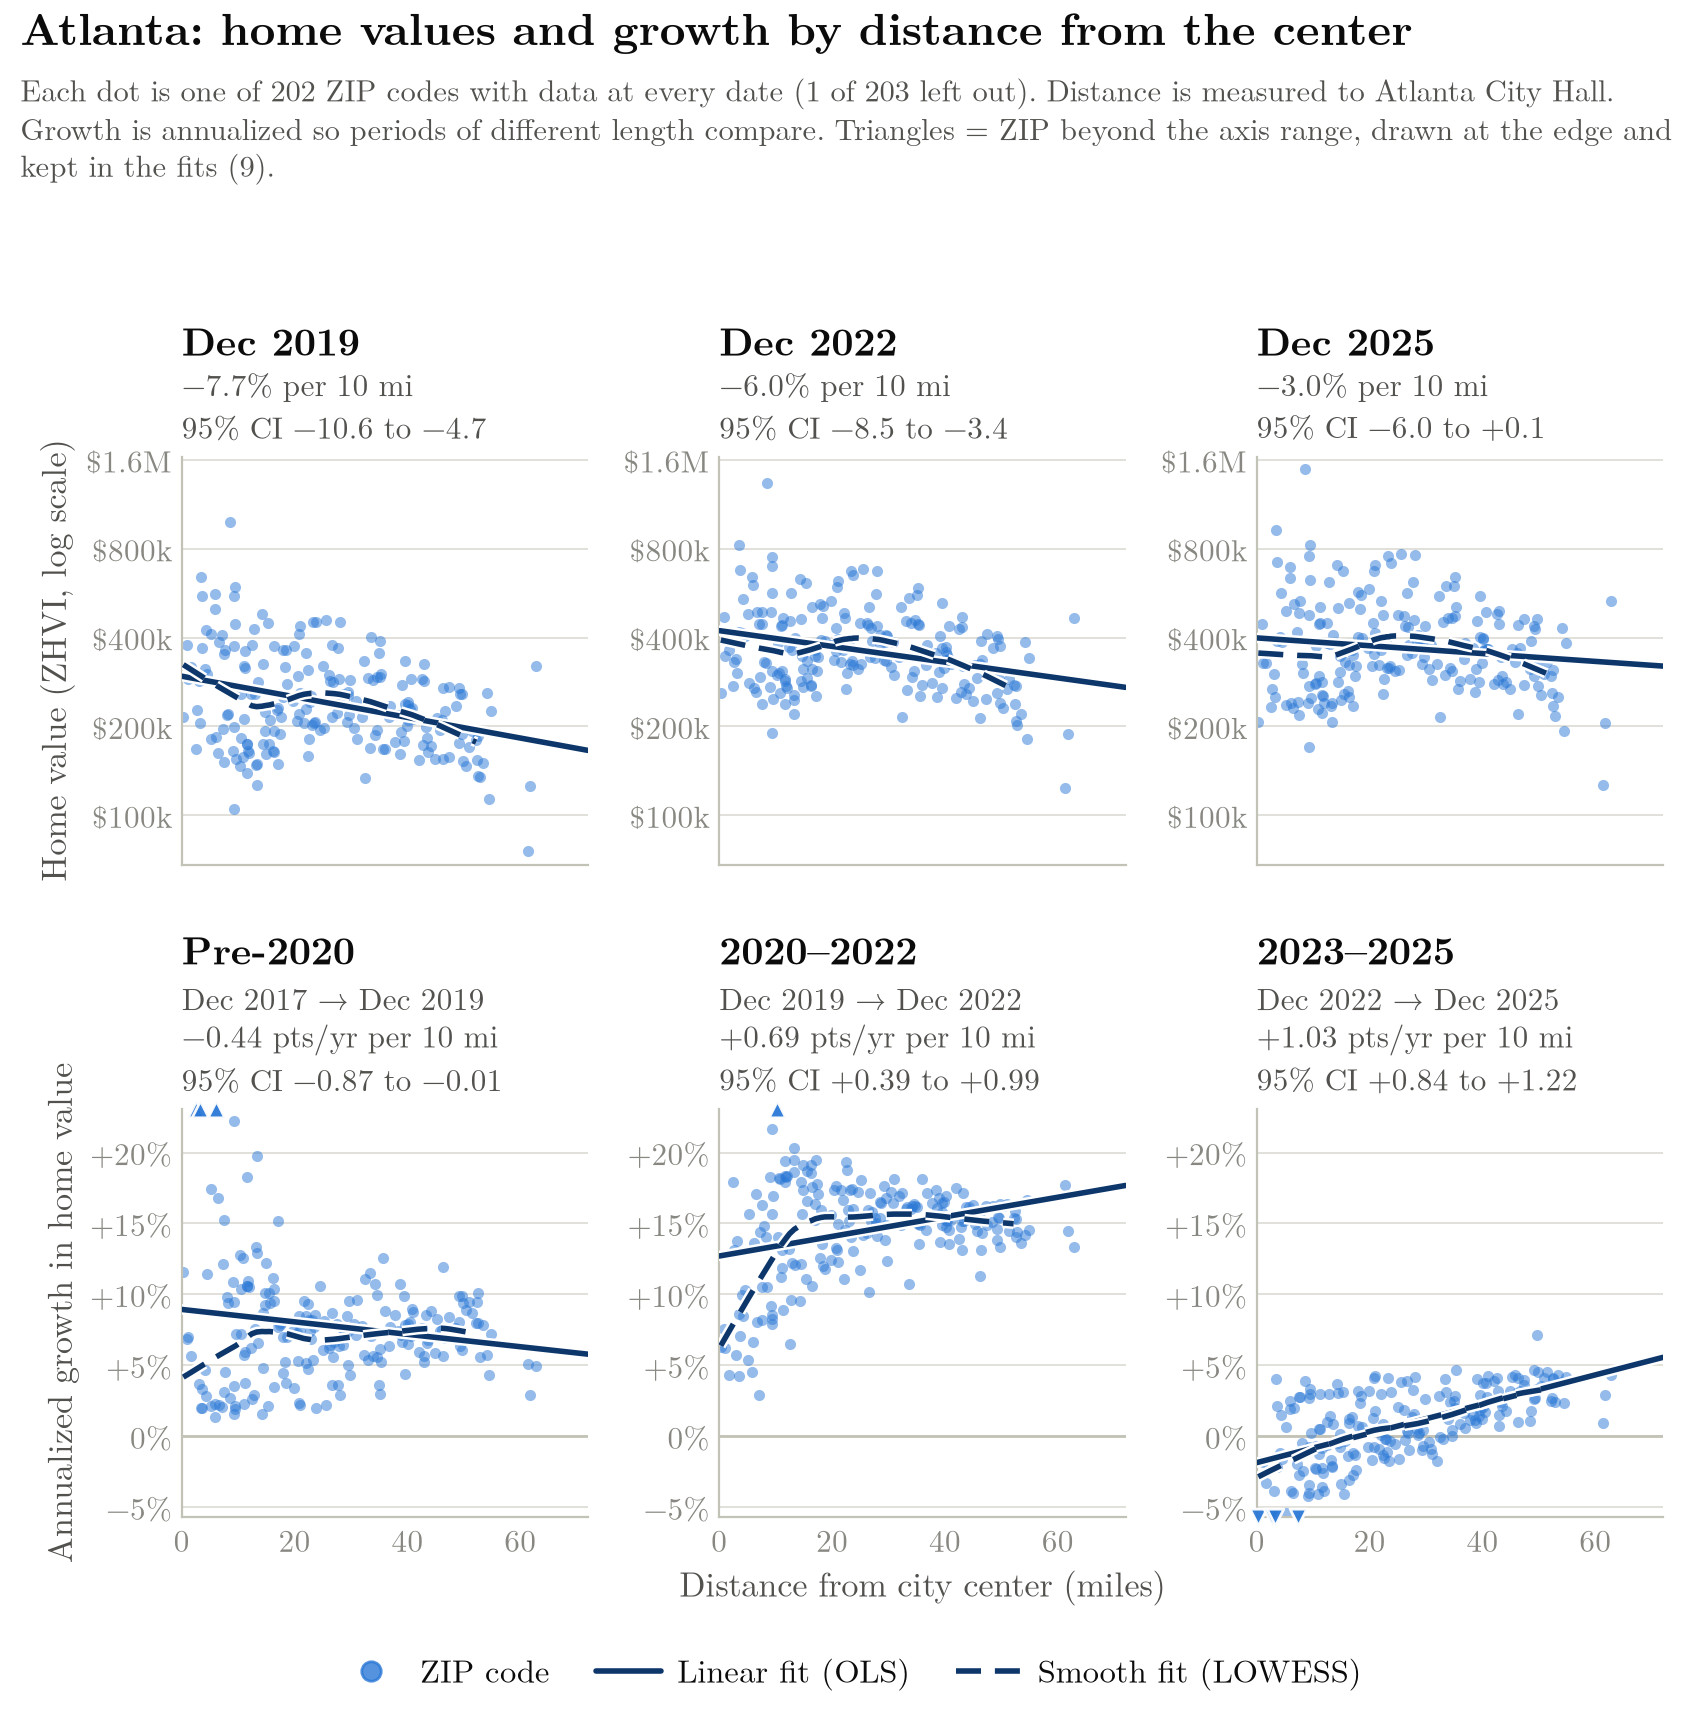
\includegraphics[width=.49\linewidth]{2_2_gradient_atlanta}\hfill
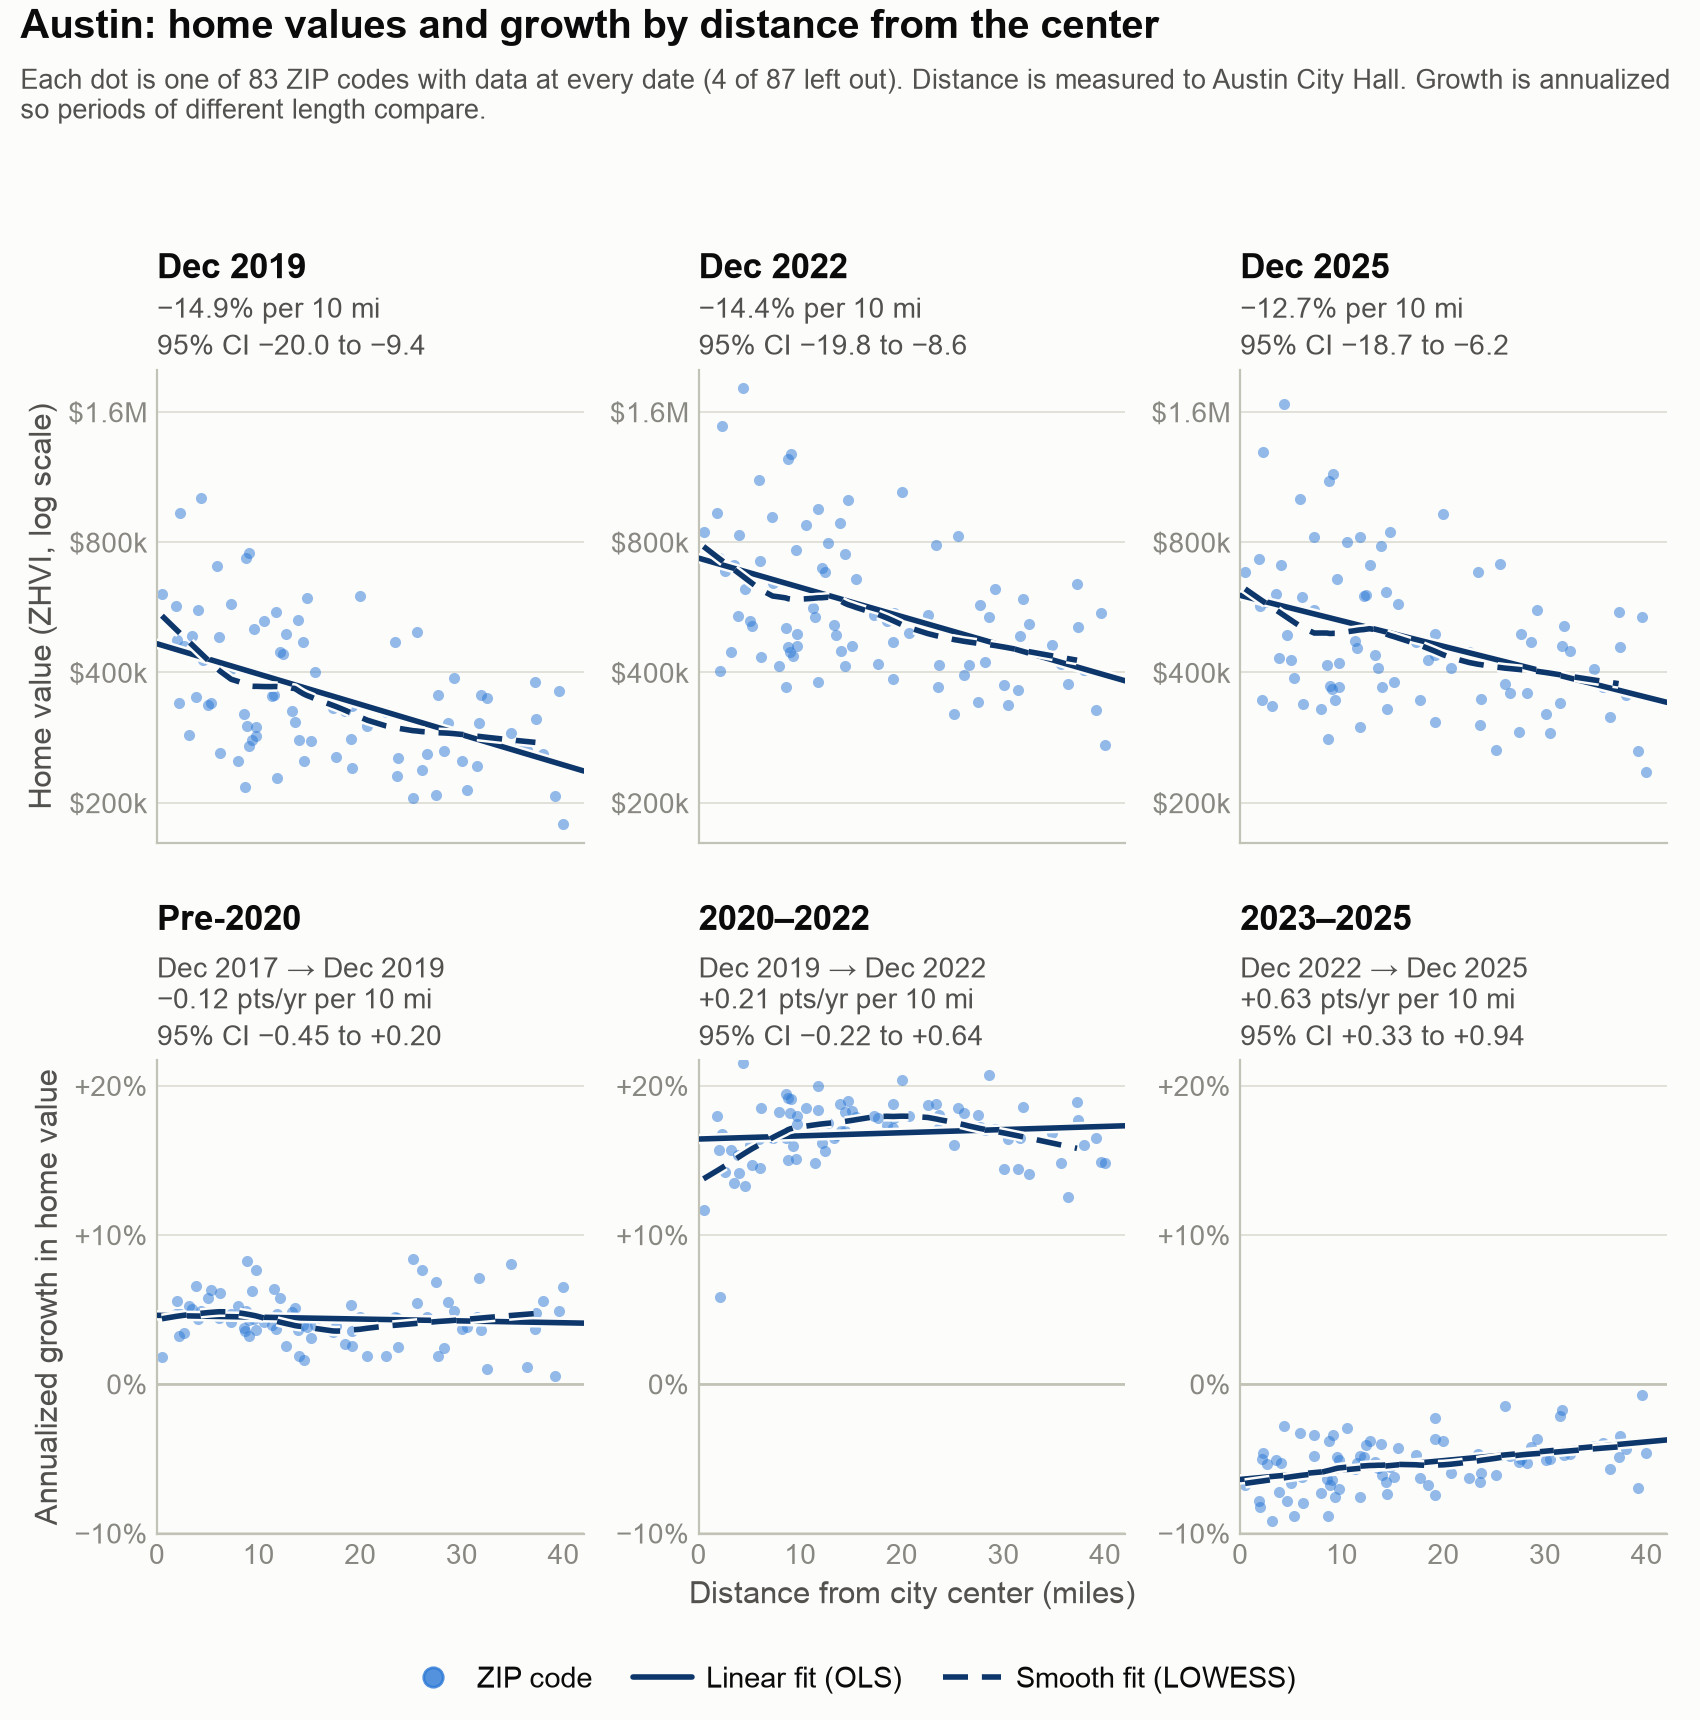
\includegraphics[width=.49\linewidth]{2_2_gradient_austin}\par\vspace{5pt}
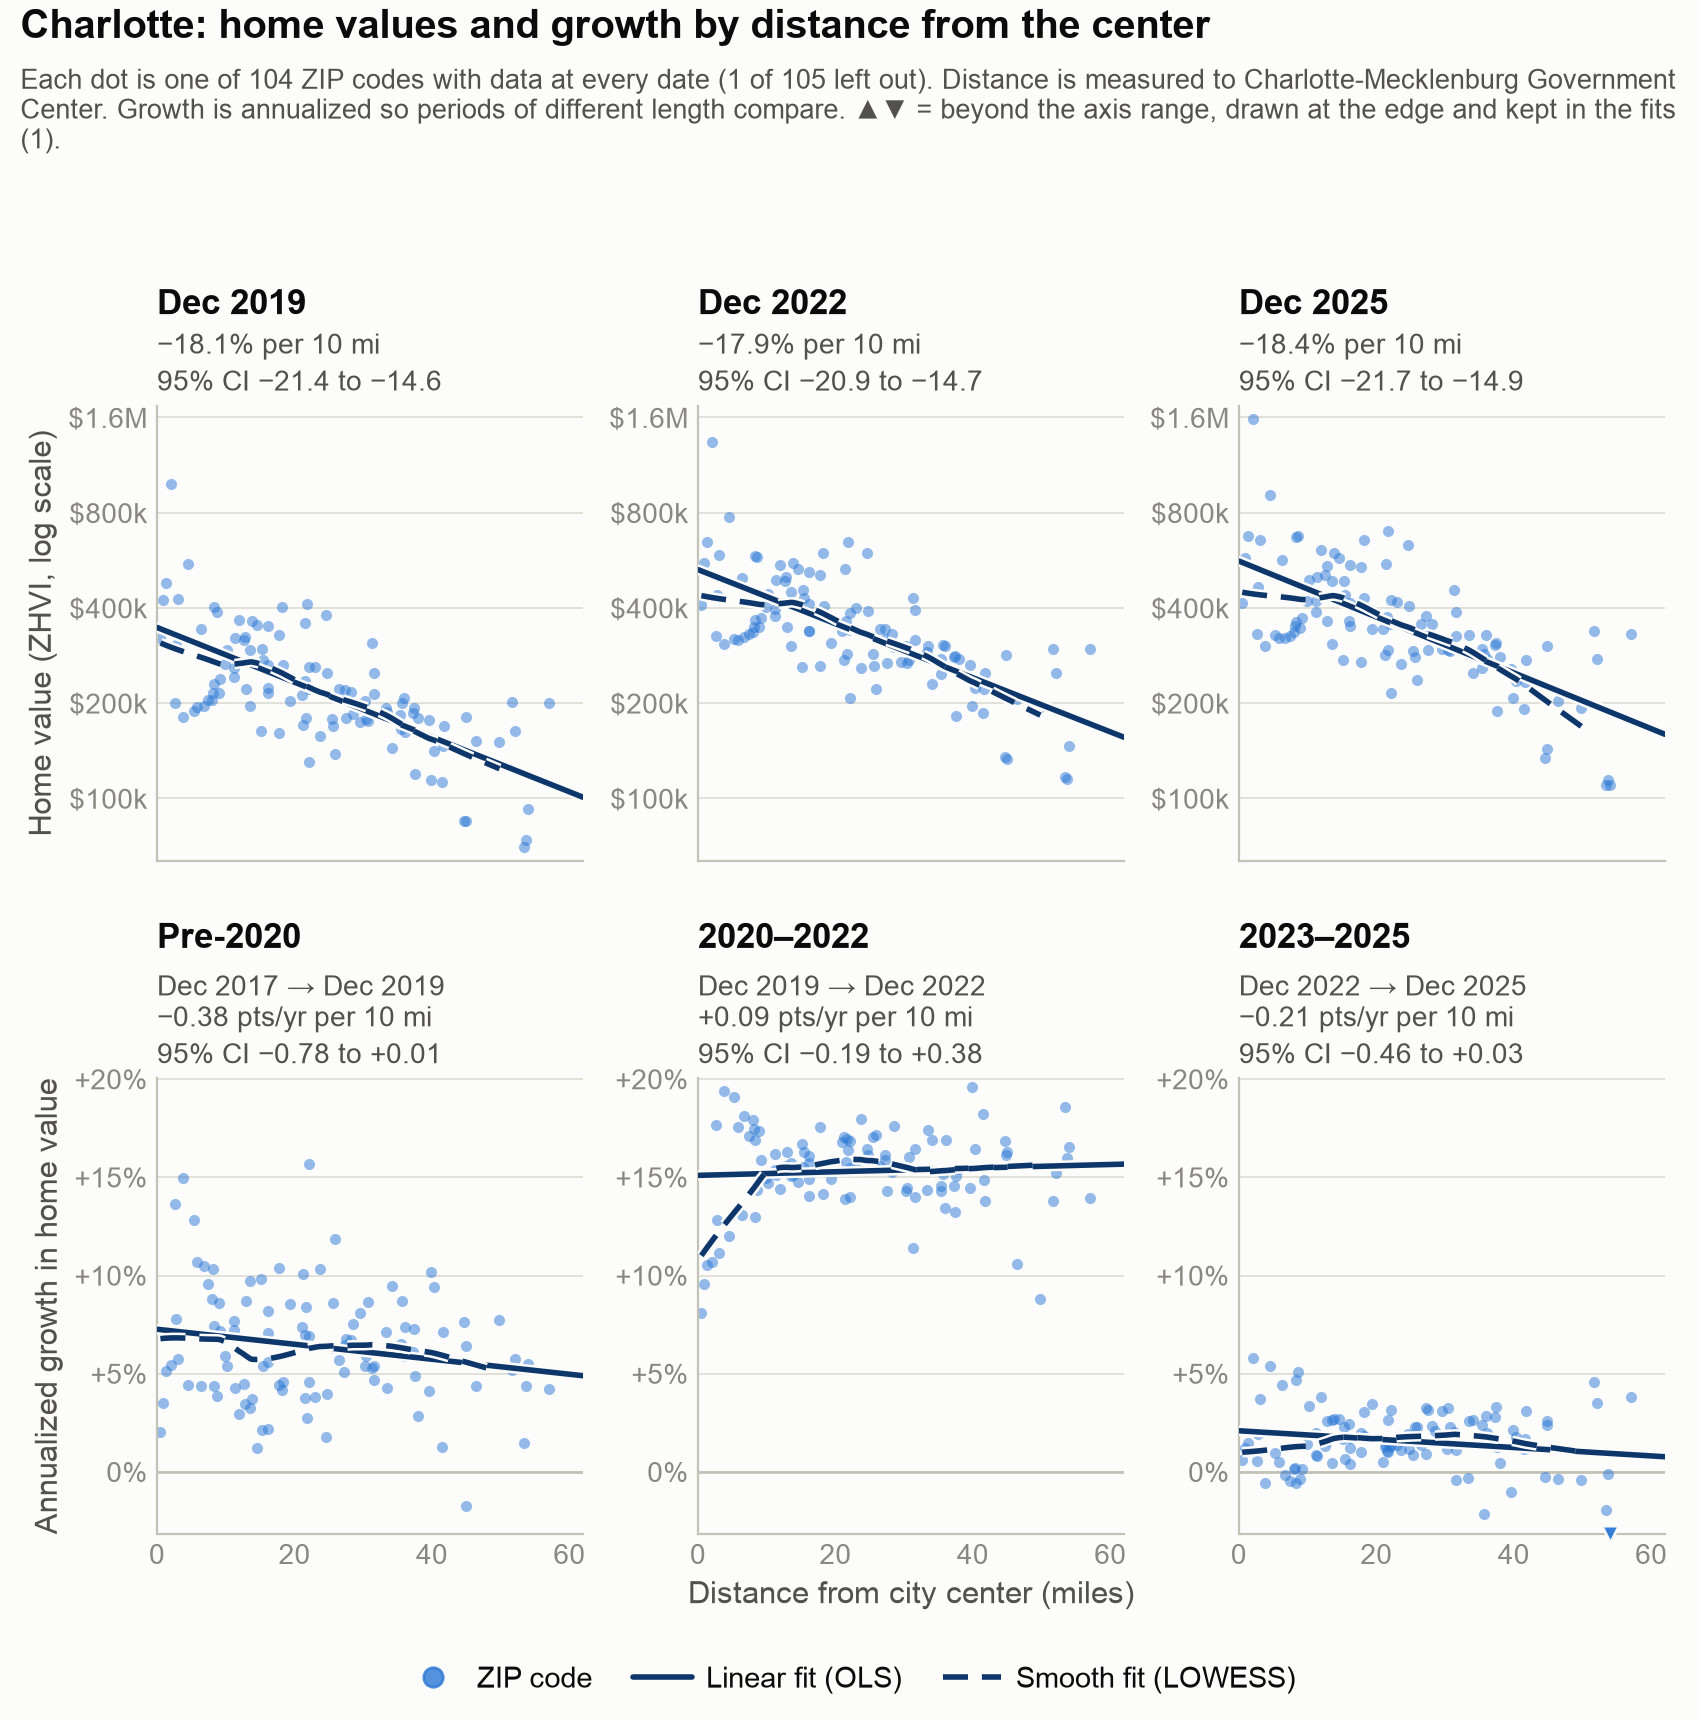
\includegraphics[width=.49\linewidth]{2_2_gradient_charlotte}\hfill
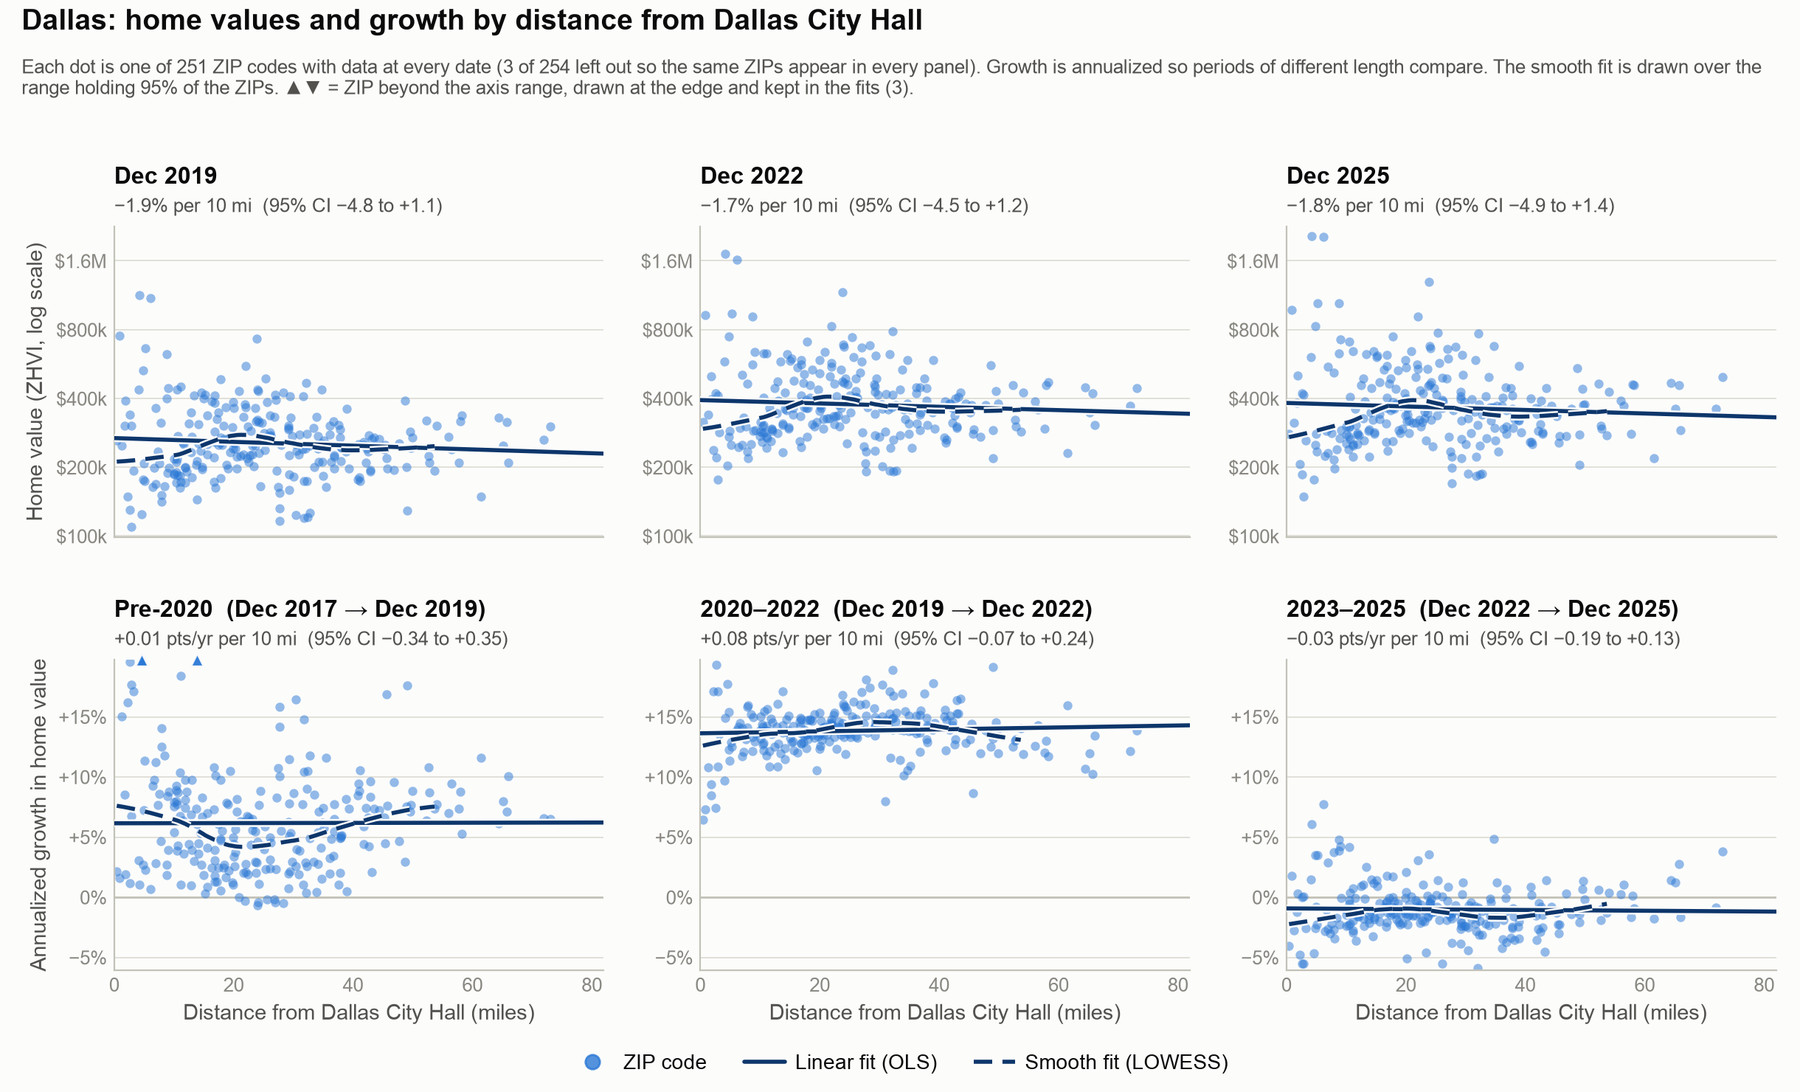
\includegraphics[width=.49\linewidth]{2_2_gradient_dallas}\par\vspace{4pt}
\refstepcounter{fignum}\label{fig:metrograd1}
{\small\raggedright\textbf{Figure \thefignum.} Price levels and period growth against distance for Atlanta, Austin, Charlotte, and
Dallas. Linear slopes provide the reported summary; smooth curves reveal nonlinearities and sparse outer-distance support.\par
\footnotesize\textit{Sources:} Zillow Research (ZHVI) and U.S. Census Bureau geography.\par}
\end{figure}

The first four panels show why the pooled average needs a metro-level reading. Atlanta has the clearest change in both the fitted
line and the smooth curve. Austin's outward pattern appears later, while Charlotte's central premium remains visible and Dallas
stays close to flat on average. The Dallas scatter also covers several submarkets, so a small overall slope should not be read as
evidence that location is unimportant within the metropolitan area.

\begin{figure}[H]\centering
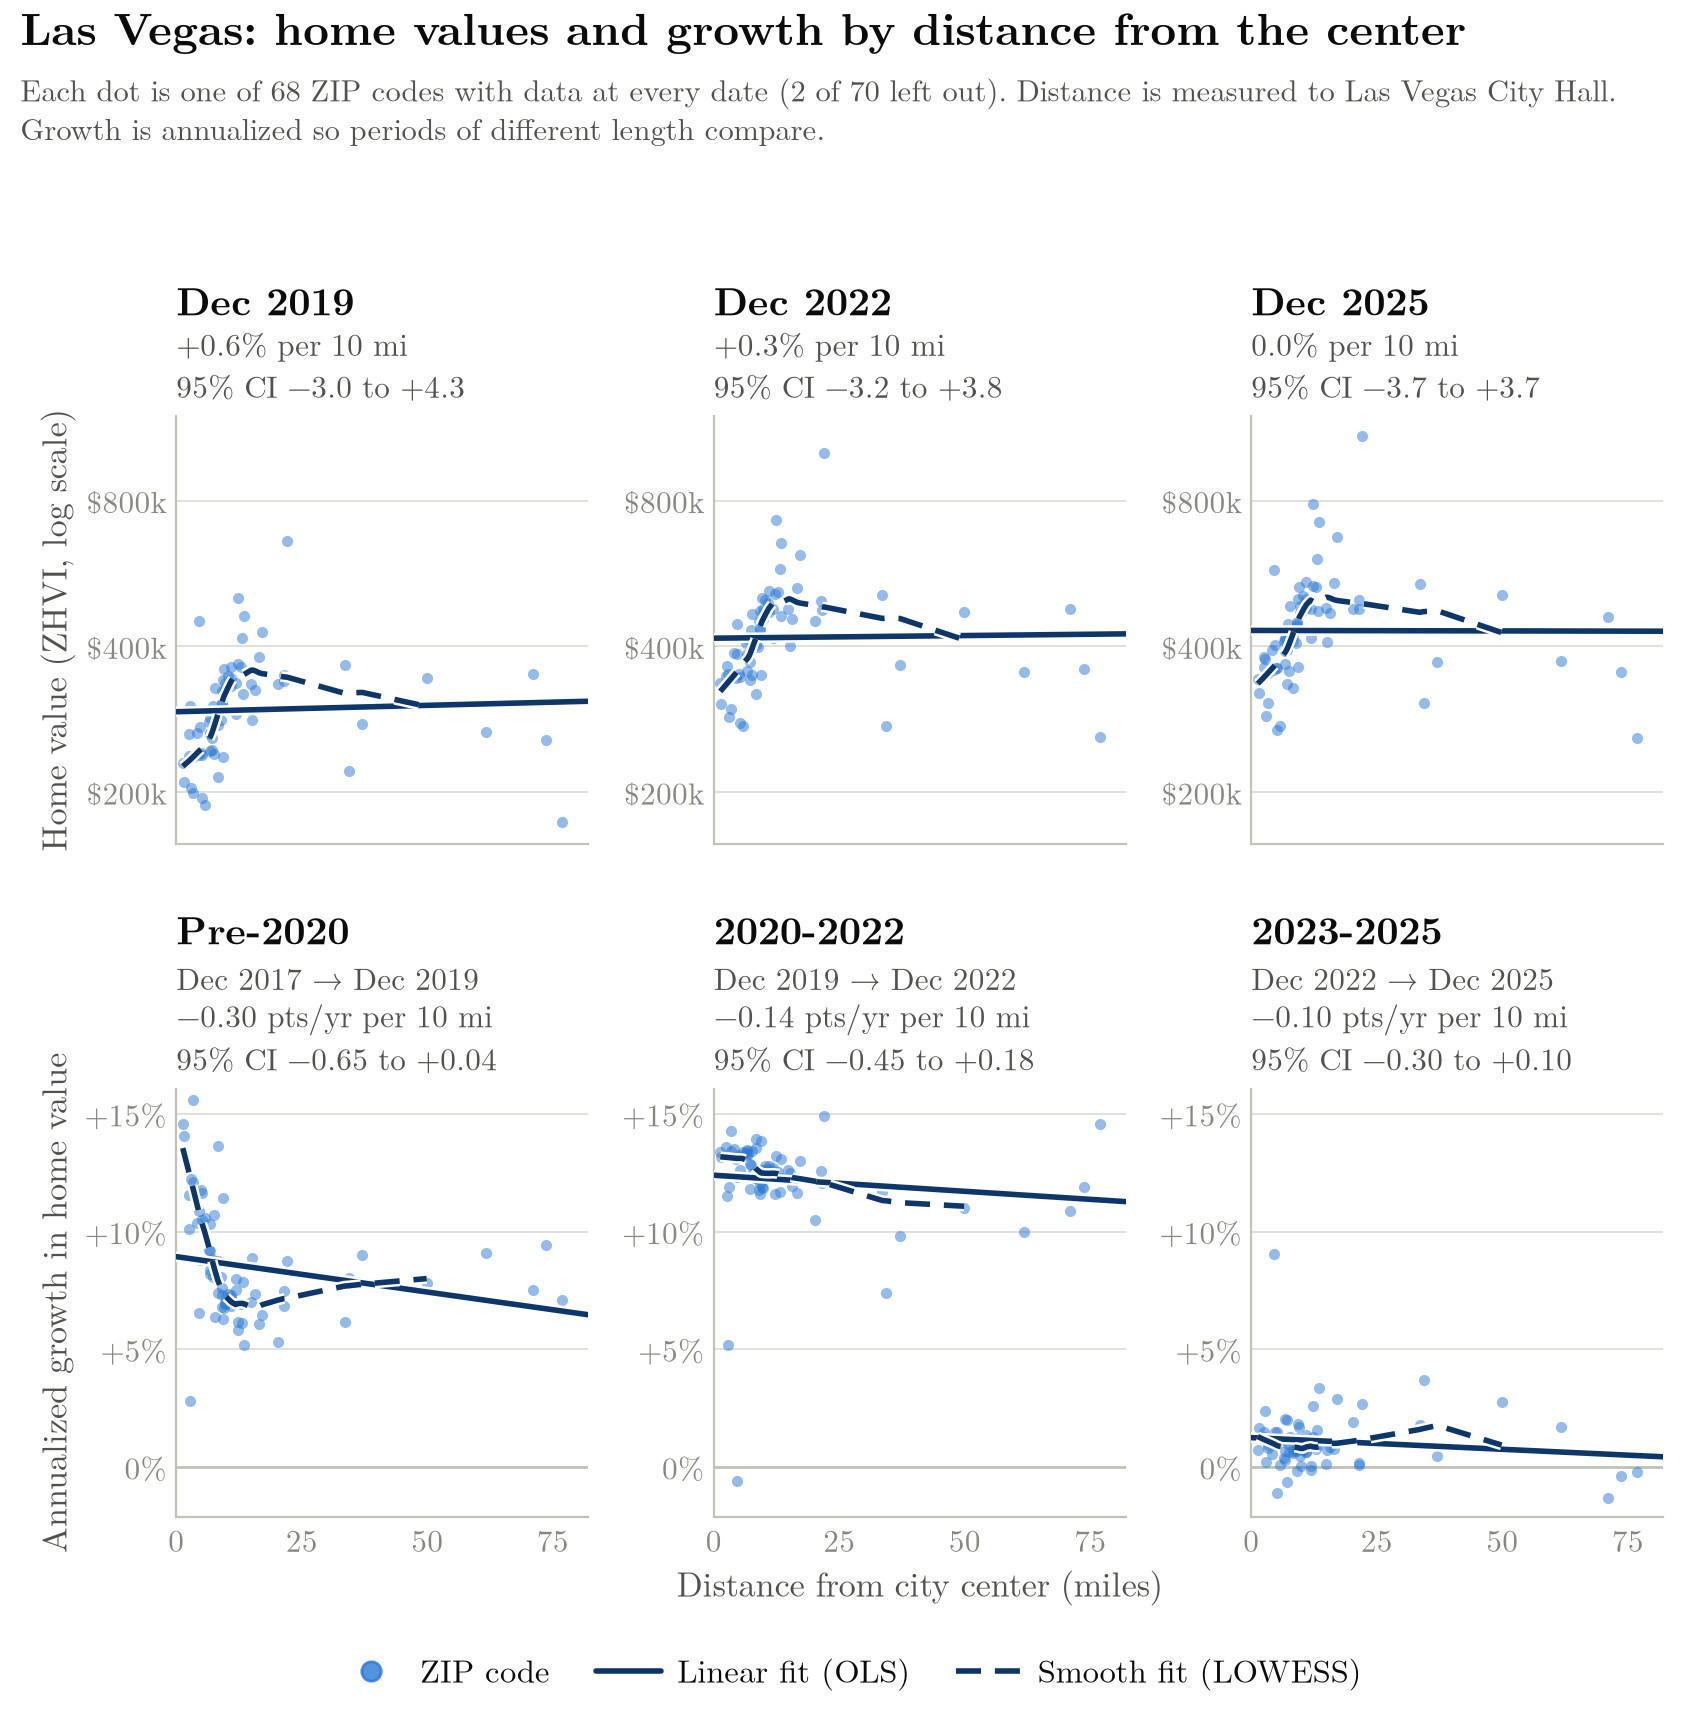
\includegraphics[width=.475\linewidth]{2_2_gradient_las_vegas}\hfill
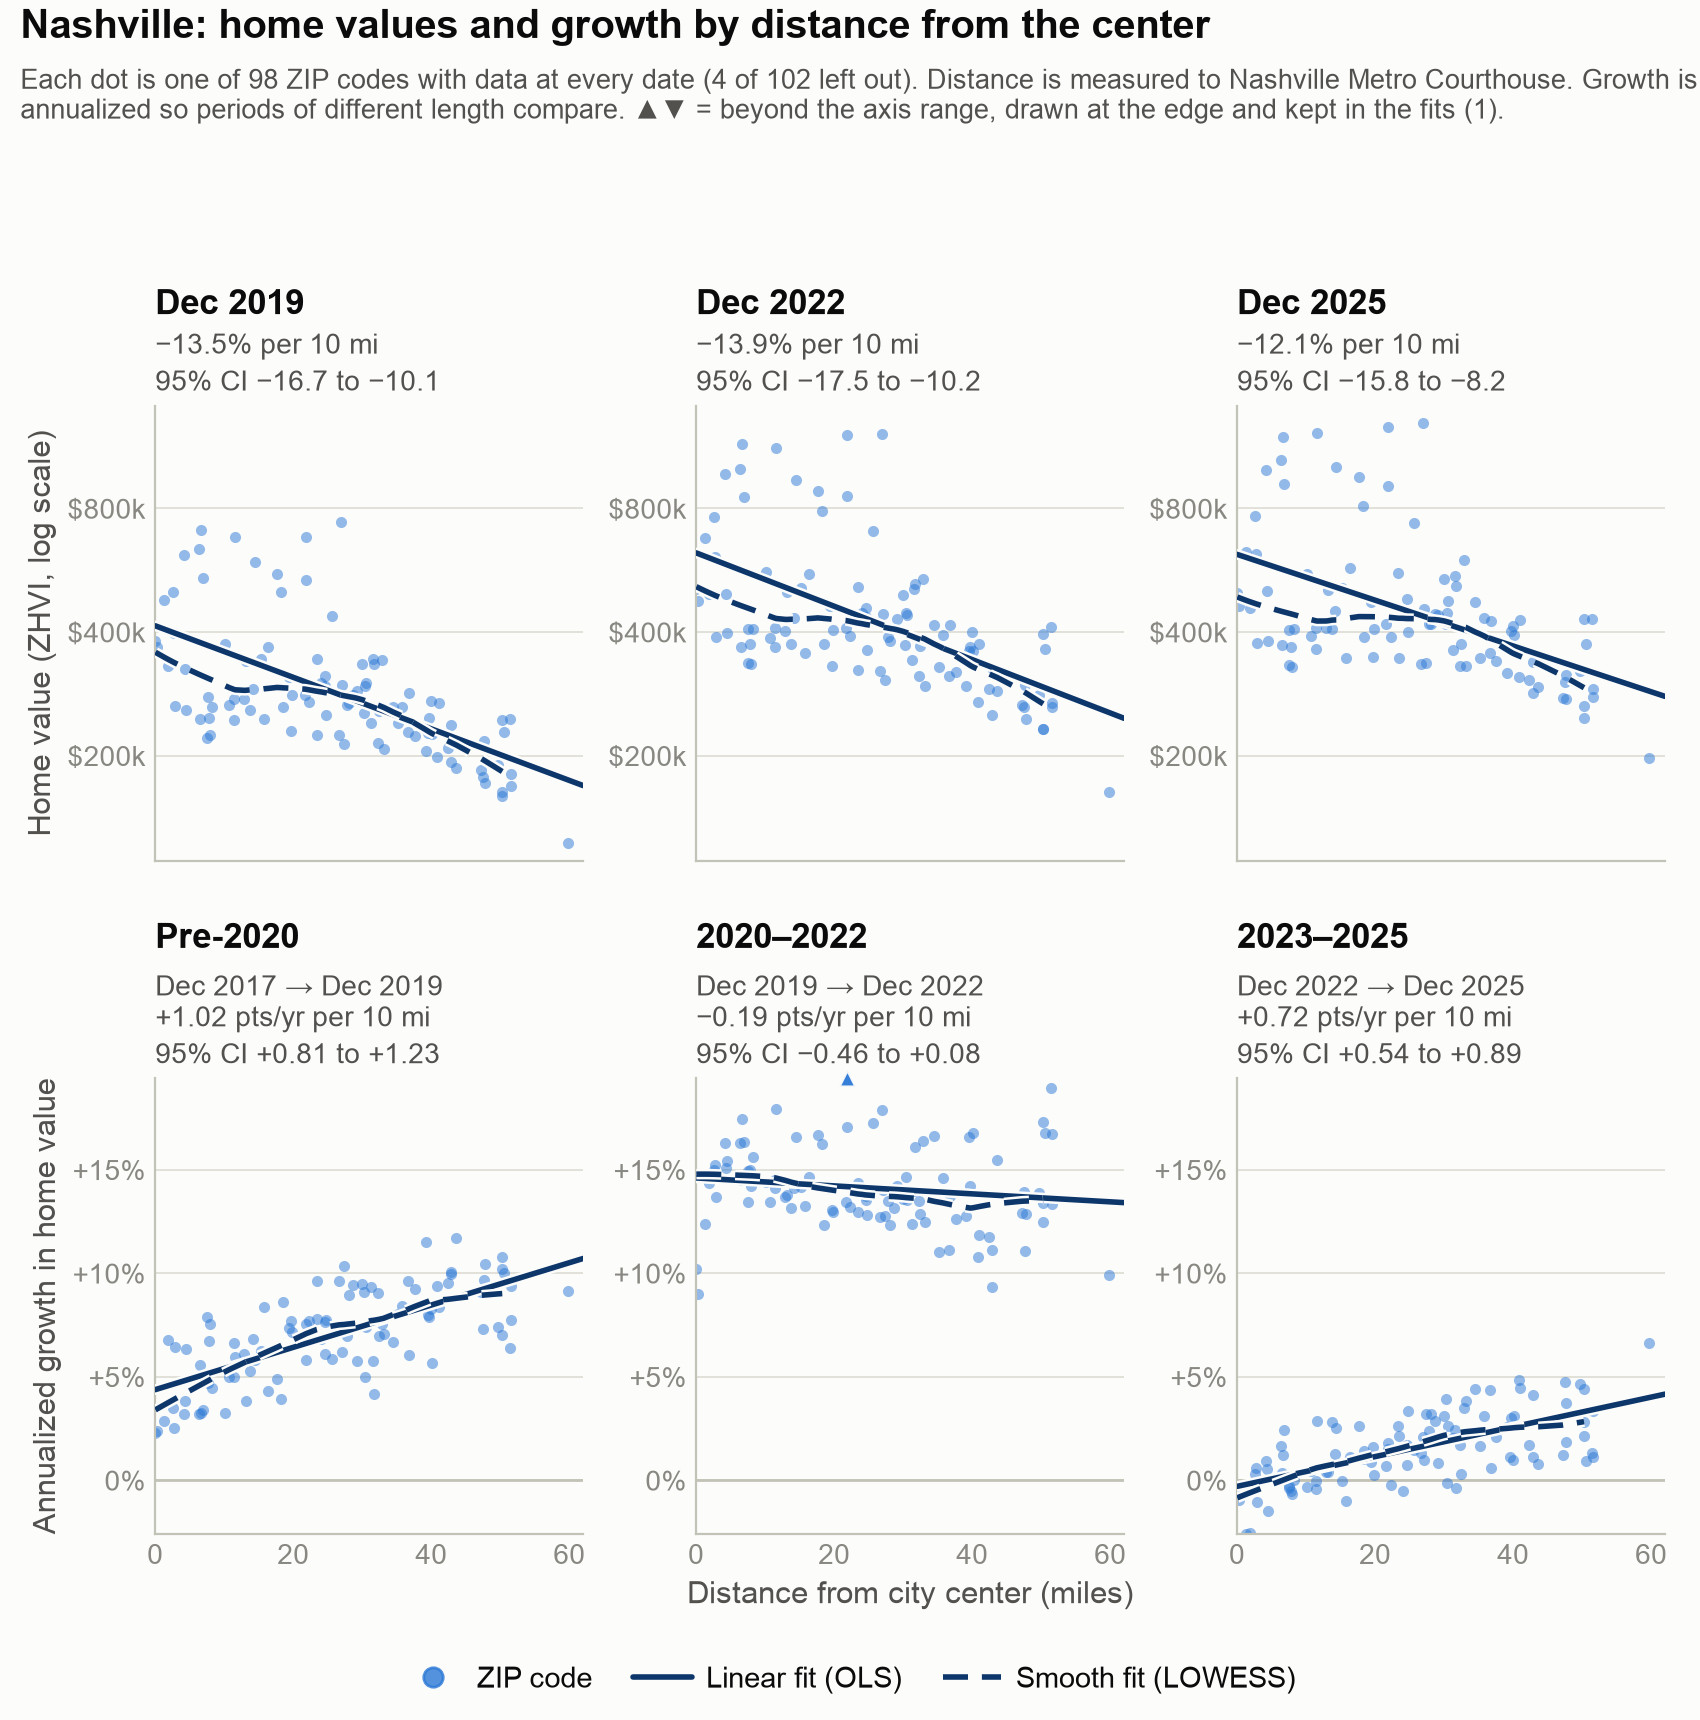
\includegraphics[width=.475\linewidth]{2_2_gradient_nashville}\par\vspace{3pt}
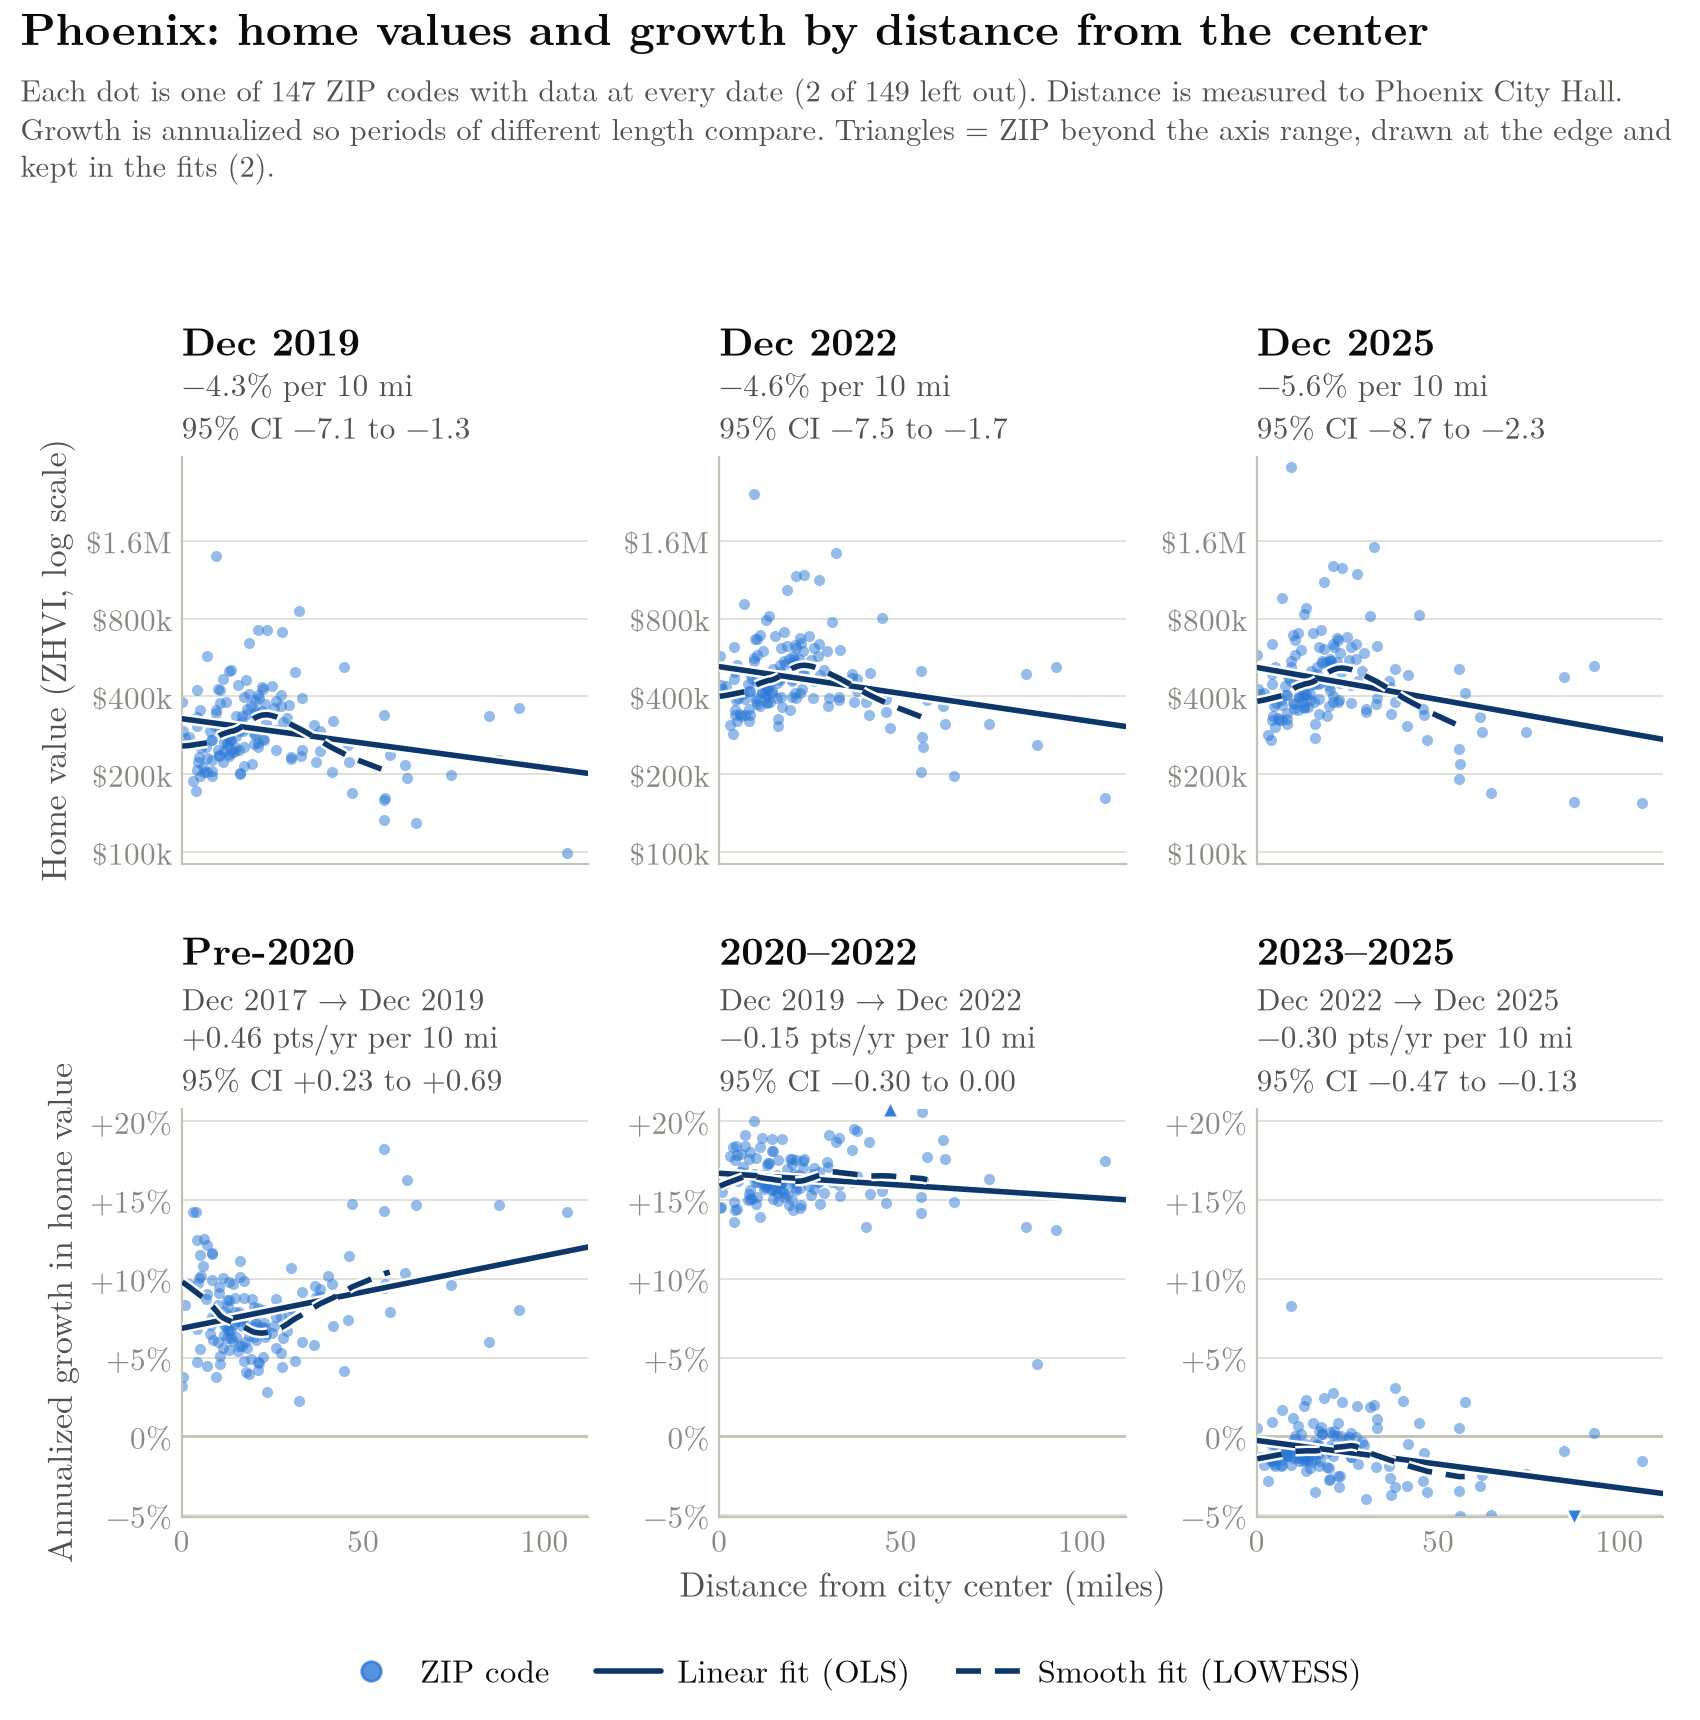
\includegraphics[width=.475\linewidth]{2_2_gradient_phoenix}\hfill
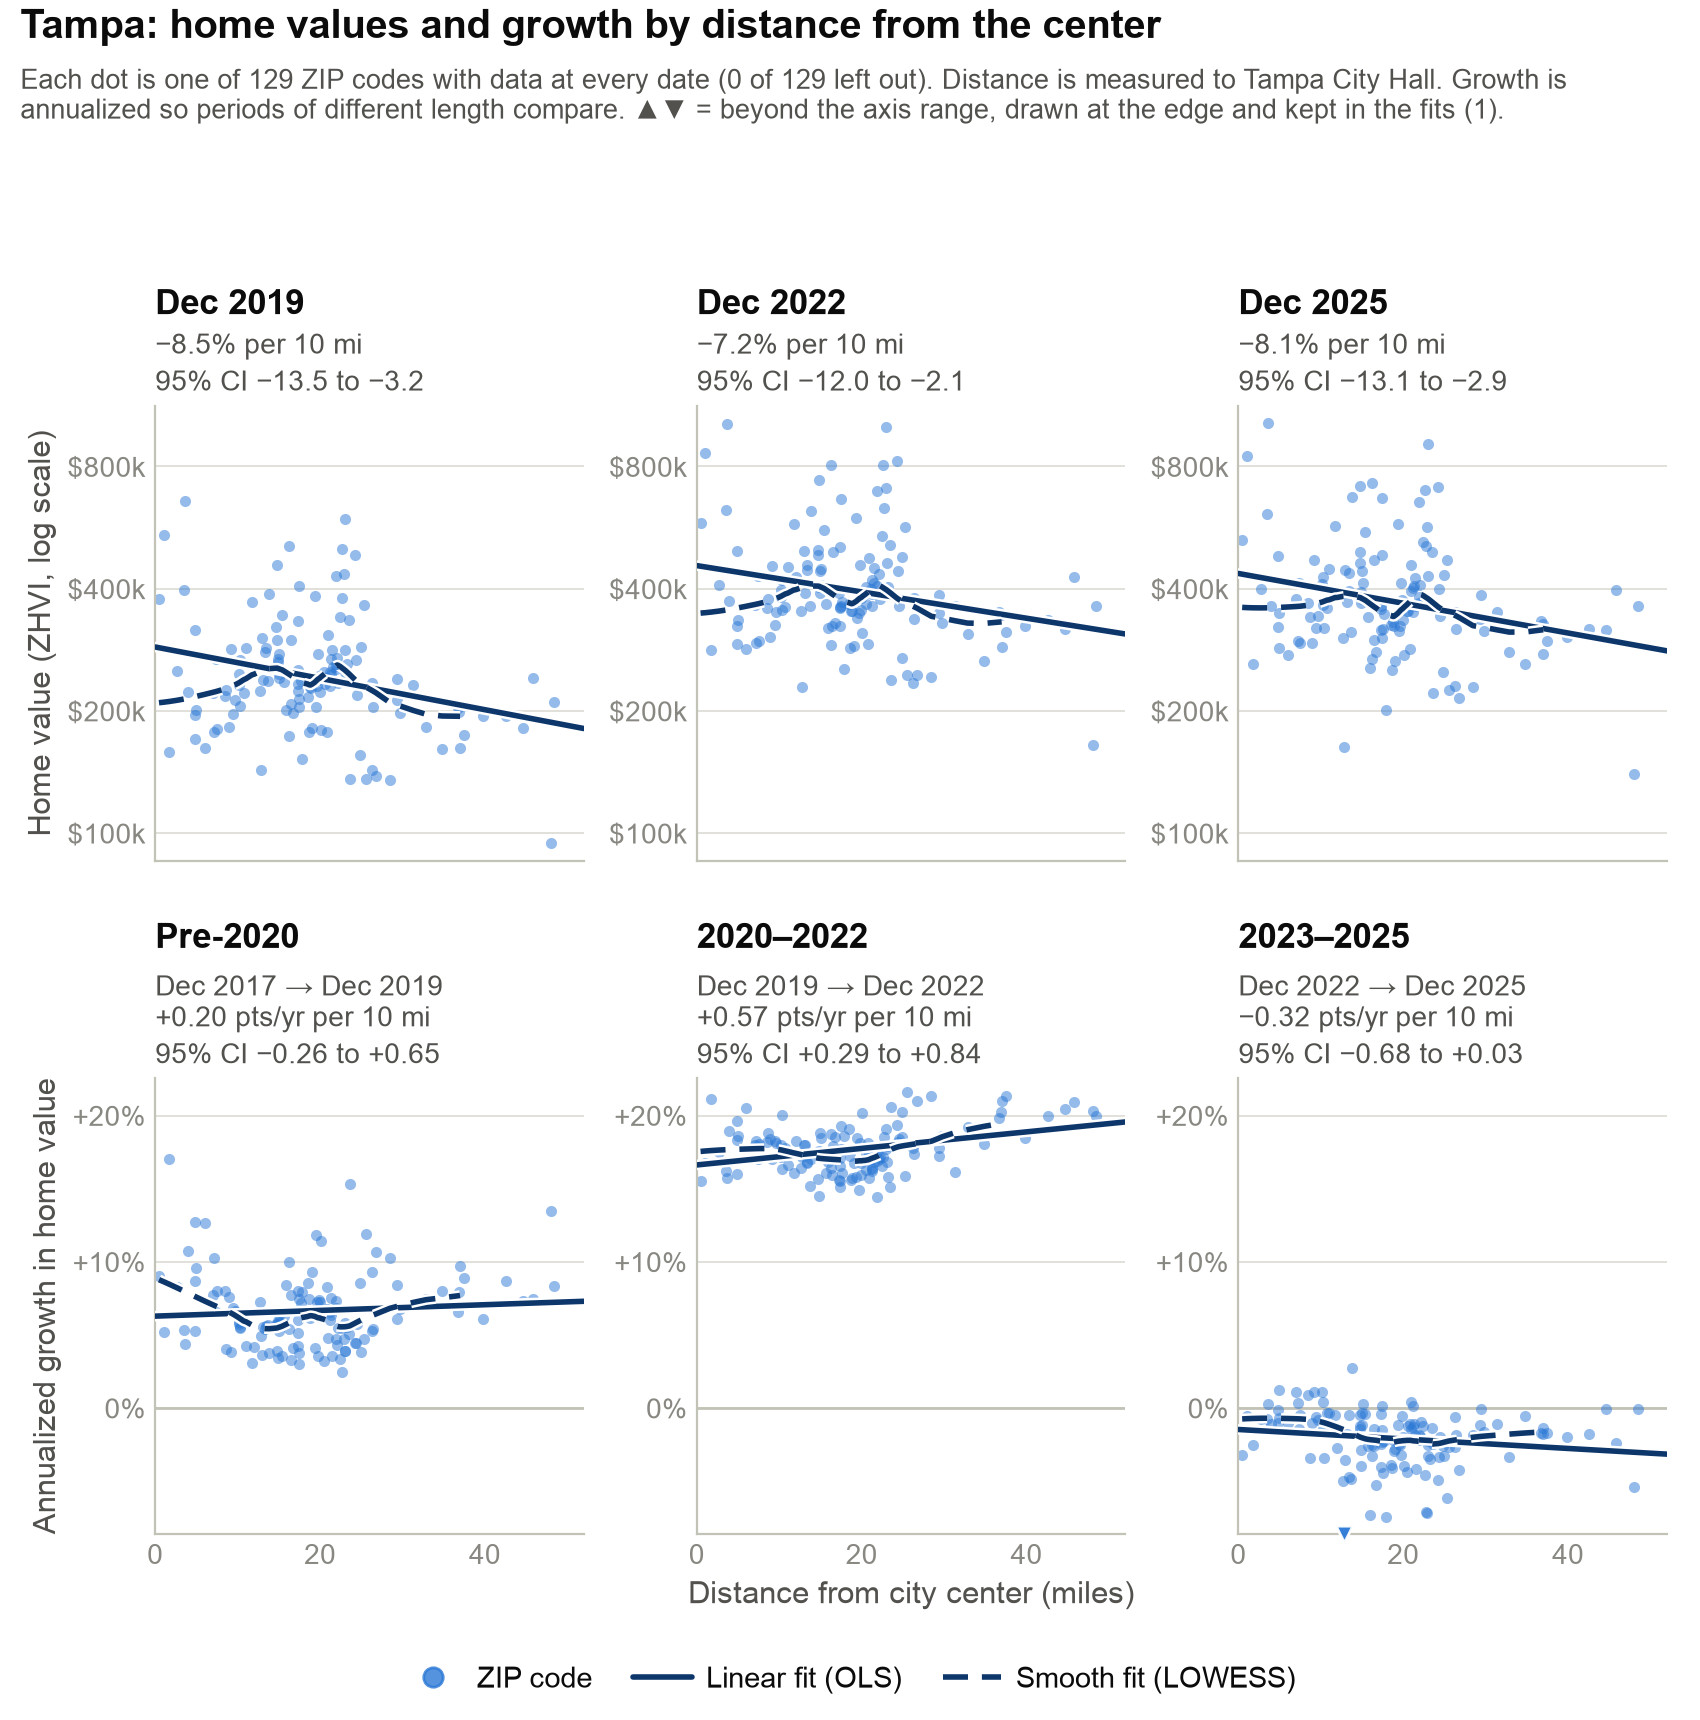
\includegraphics[width=.475\linewidth]{2_2_gradient_tampa}\par\vspace{3pt}
\refstepcounter{fignum}\label{fig:metrograd2}
{\small\raggedright\textbf{Figure \thefignum.} Price levels and period growth against distance for Las Vegas, Nashville, Phoenix,
and Tampa. The weak or sensitive relationships and Nashville pre-trend qualify a general post-pandemic flattening claim.\par
\footnotesize\textit{Sources:} Zillow Research (ZHVI) and U.S. Census Bureau geography.\par}
\end{figure}

\section{Two-Center Robustness}

The formal event, exposure, and prediction models use distance to the nearer named city hall. The exploratory figures begin with
the first-named city hall and then show each center separately in Dallas-Fort Worth and Tampa-St. Petersburg. This makes it possible
to see exactly which descriptive result depends on choosing one downtown.

\begin{figure}[H]\centering
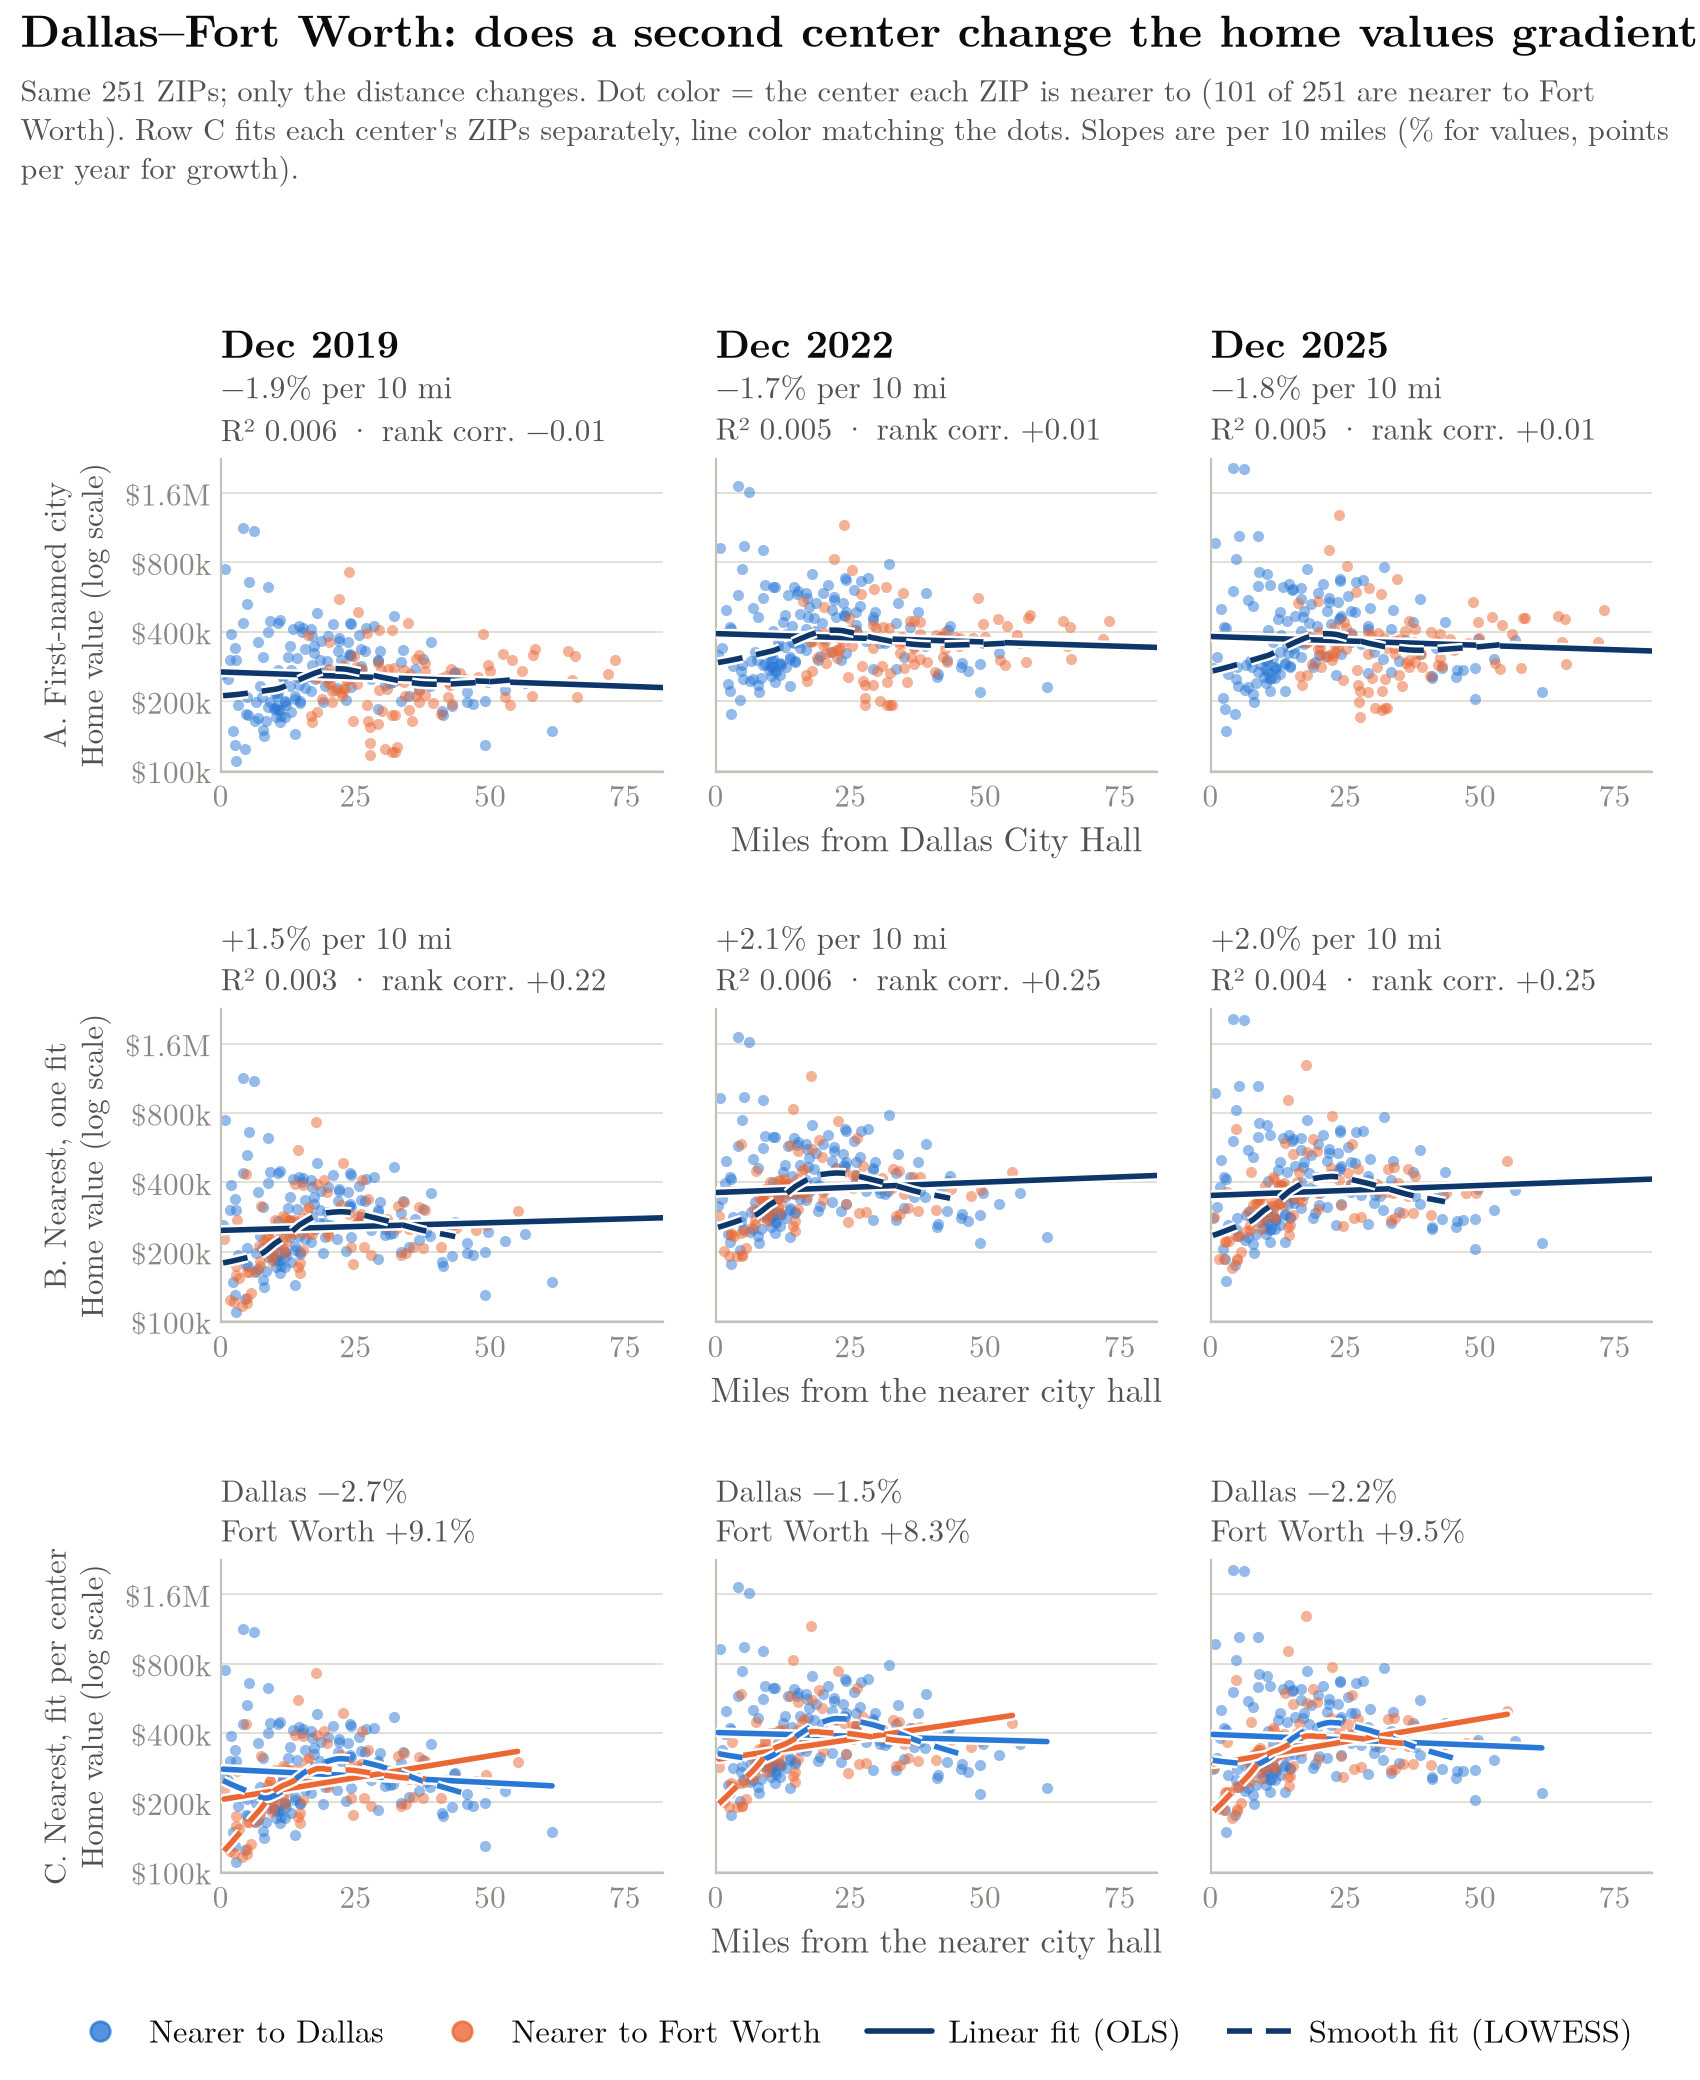
\includegraphics[width=.49\linewidth]{2_2_two_center_level_dallas}\hfill
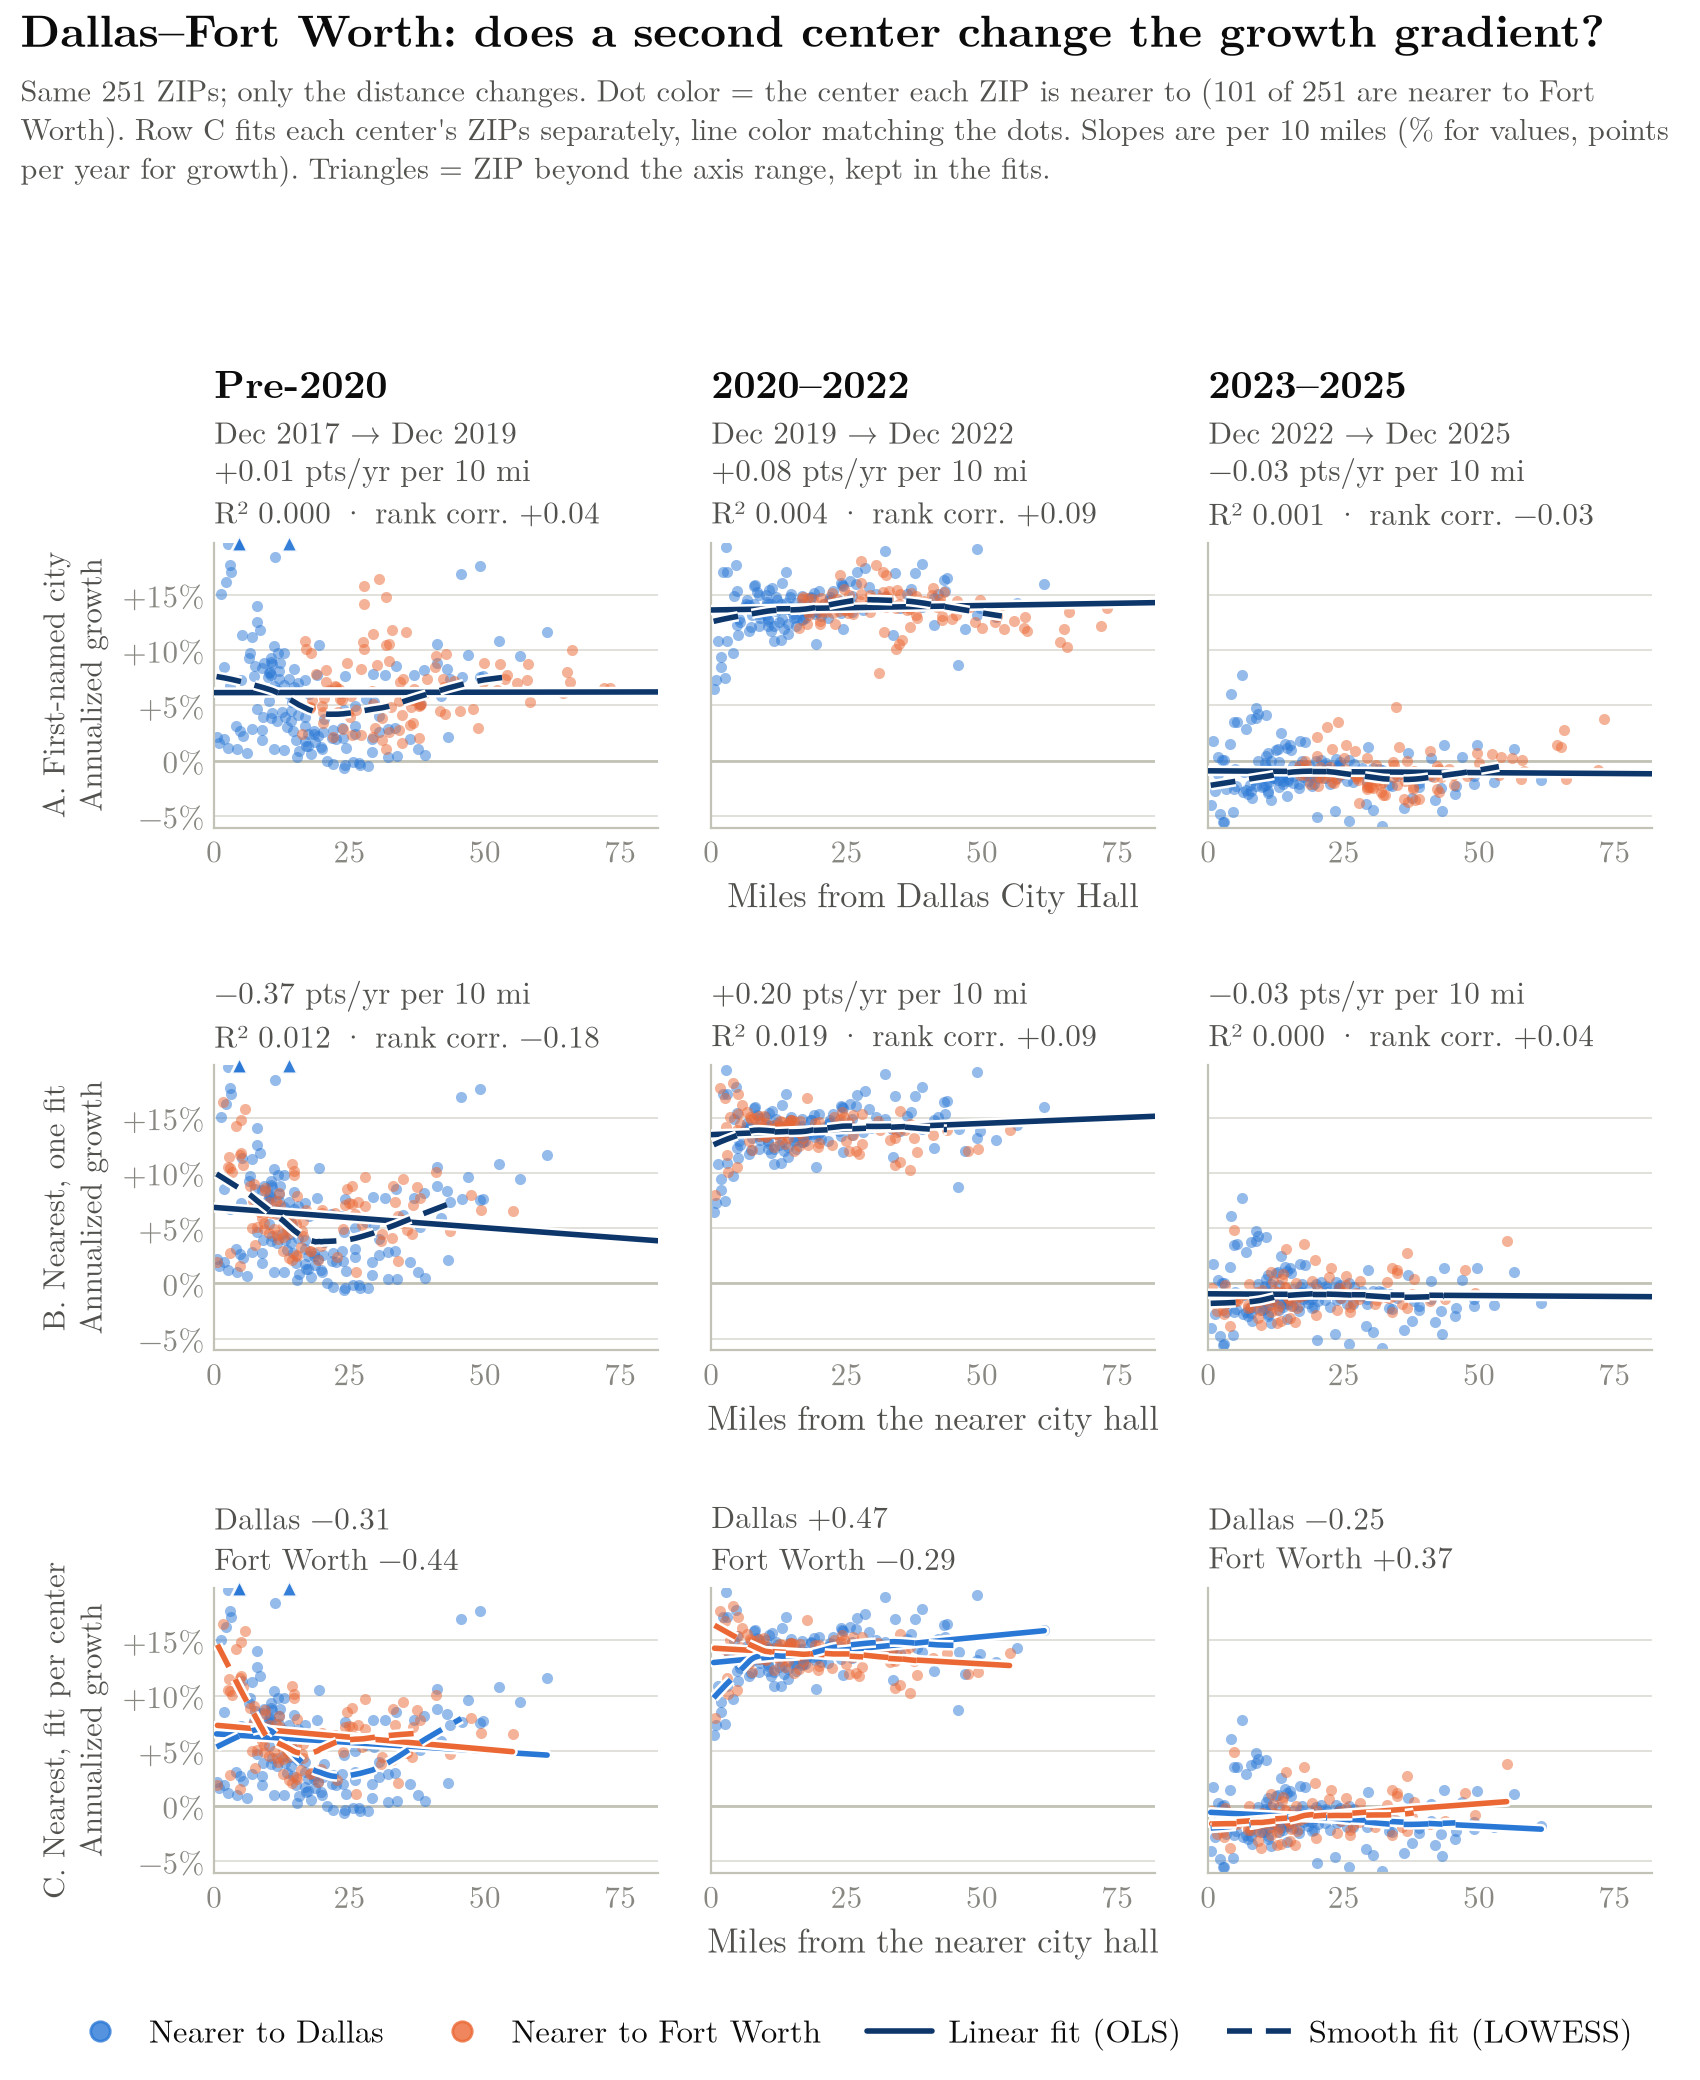
\includegraphics[width=.49\linewidth]{2_2_two_center_growth_dallas}\par\vspace{4pt}
\refstepcounter{fignum}\label{fig:twocenterDallas}
{\small\raggedright\textbf{Figure \thefignum.} Dallas-Fort Worth level and growth fits measured from Dallas, Fort Worth, and the
nearer city hall. Dallas and Fort Worth have different local price surfaces, so the second center does not restore one common
monocentric gradient.\par
\footnotesize\textit{Sources:} Zillow Research (ZHVI) and U.S. Census Bureau geography.\par}
\end{figure}

Dallas and Fort Worth do not share one price-distance surface: their central price levels and outward directions differ. Tampa and
St. Petersburg also show different local relationships, and Tampa's post-2022 reversal disappears when distance is measured to the
nearer center.
The better next step is to measure employment centers or travel-time access rather than adding city halls until a radial pattern
appears.

Figure~\ref{fig:twocenterDallas} separates three versions of the same comparison: distance from Dallas, distance from Fort Worth,
and distance from whichever center is closer. The fitted relationships do not converge when the nearer center is used. Instead,
the exercise shows that the two sides of the metro have different level and growth surfaces. The formal models use the nearer-center
measure, while the separate-center plots show why even that definition is an incomplete representation of access.

\begin{figure}[H]\centering
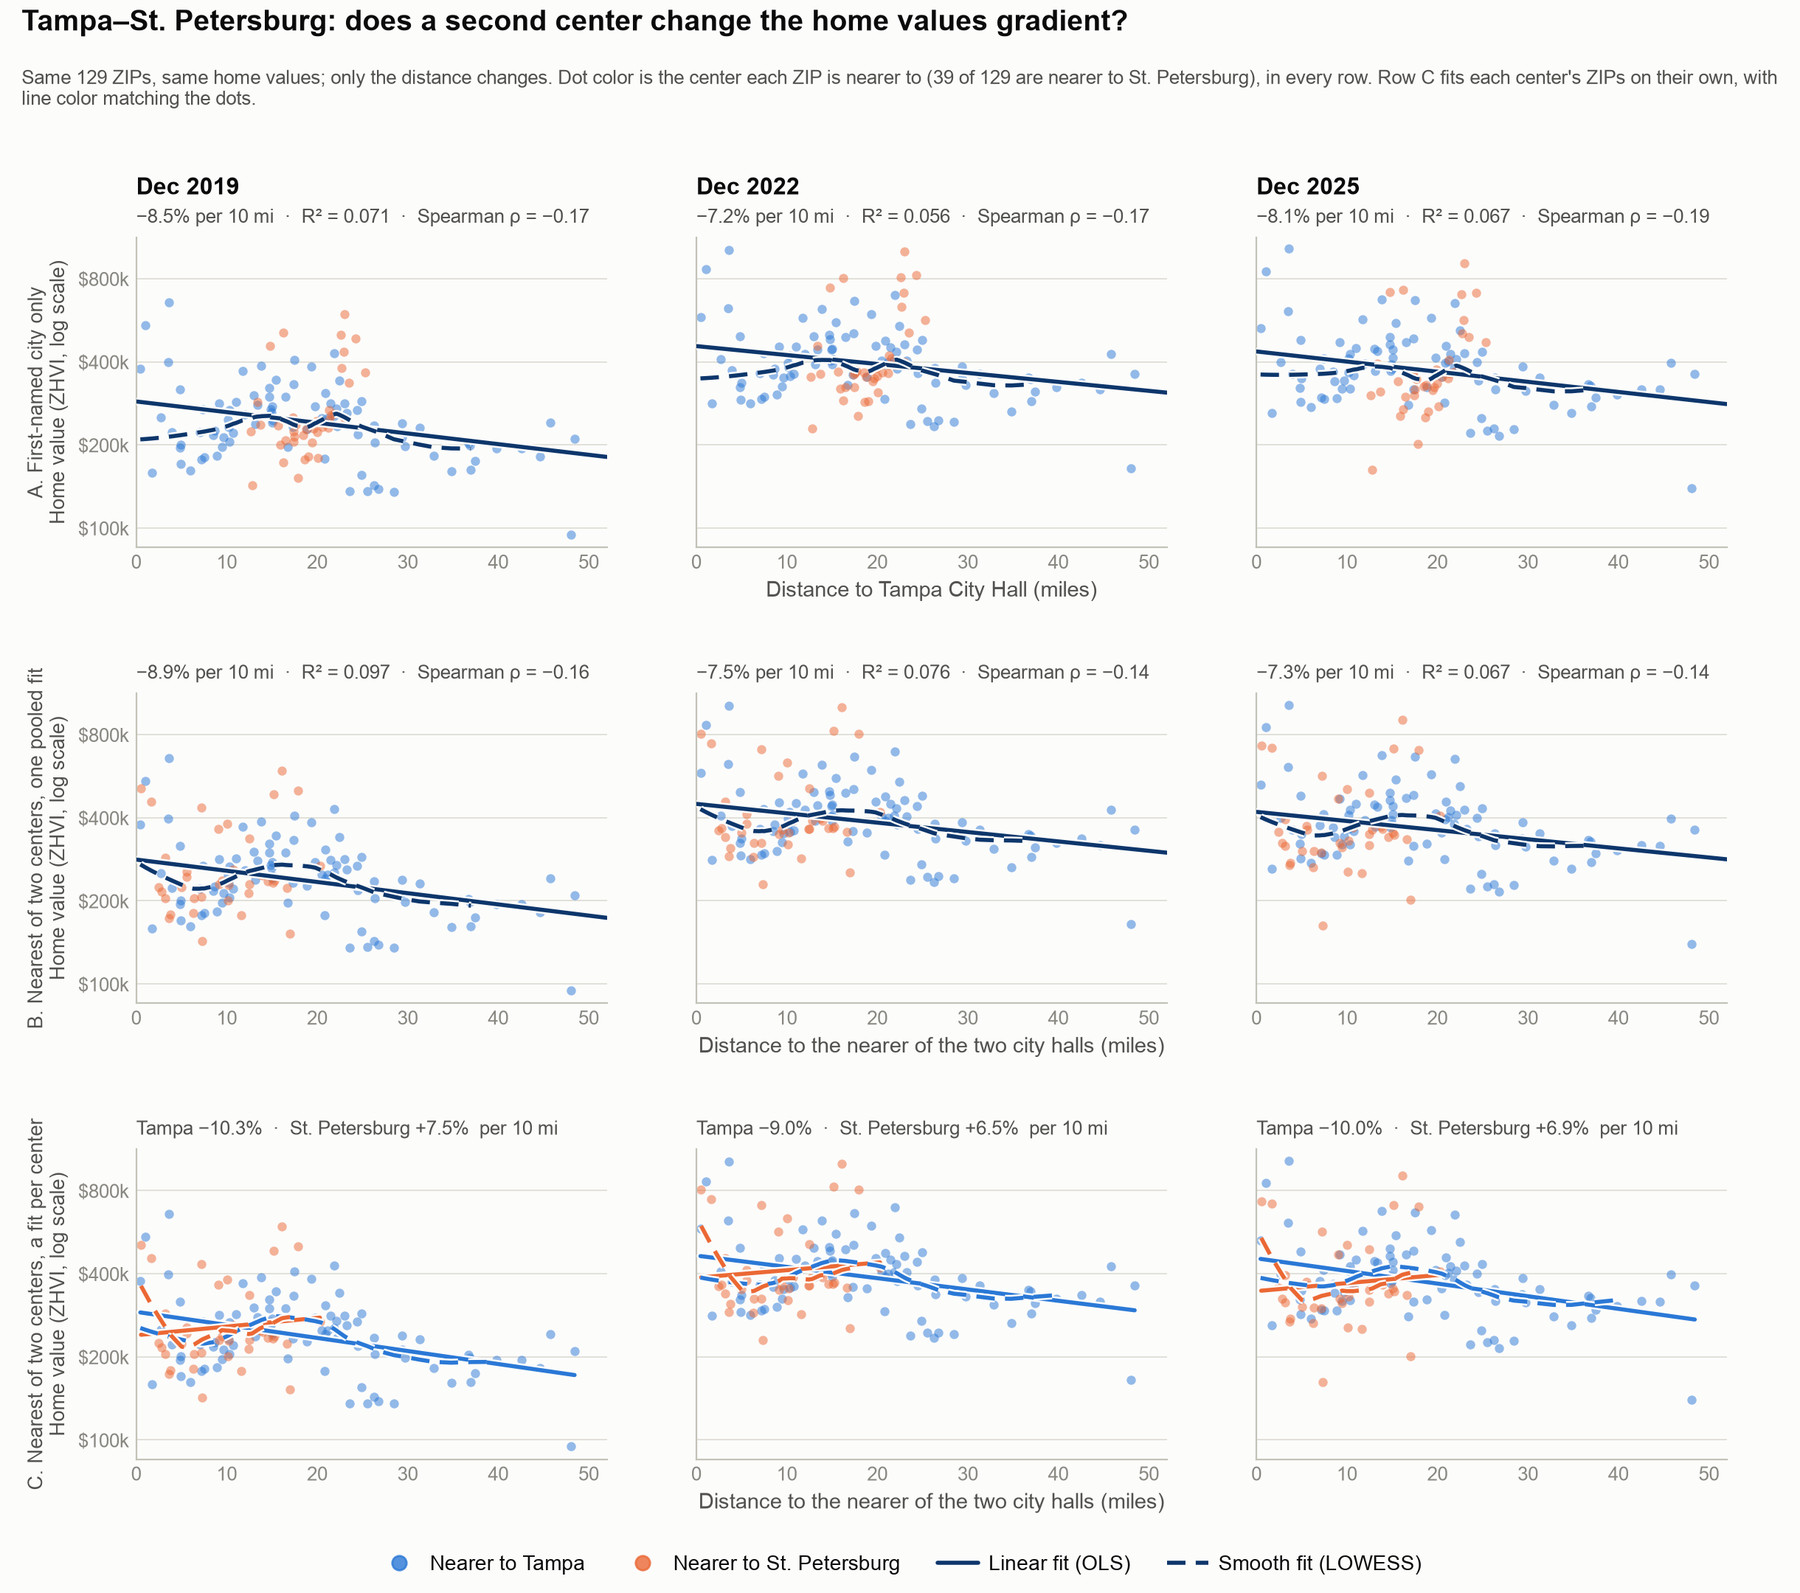
\includegraphics[width=.49\linewidth]{2_2_two_center_level_tampa}\hfill
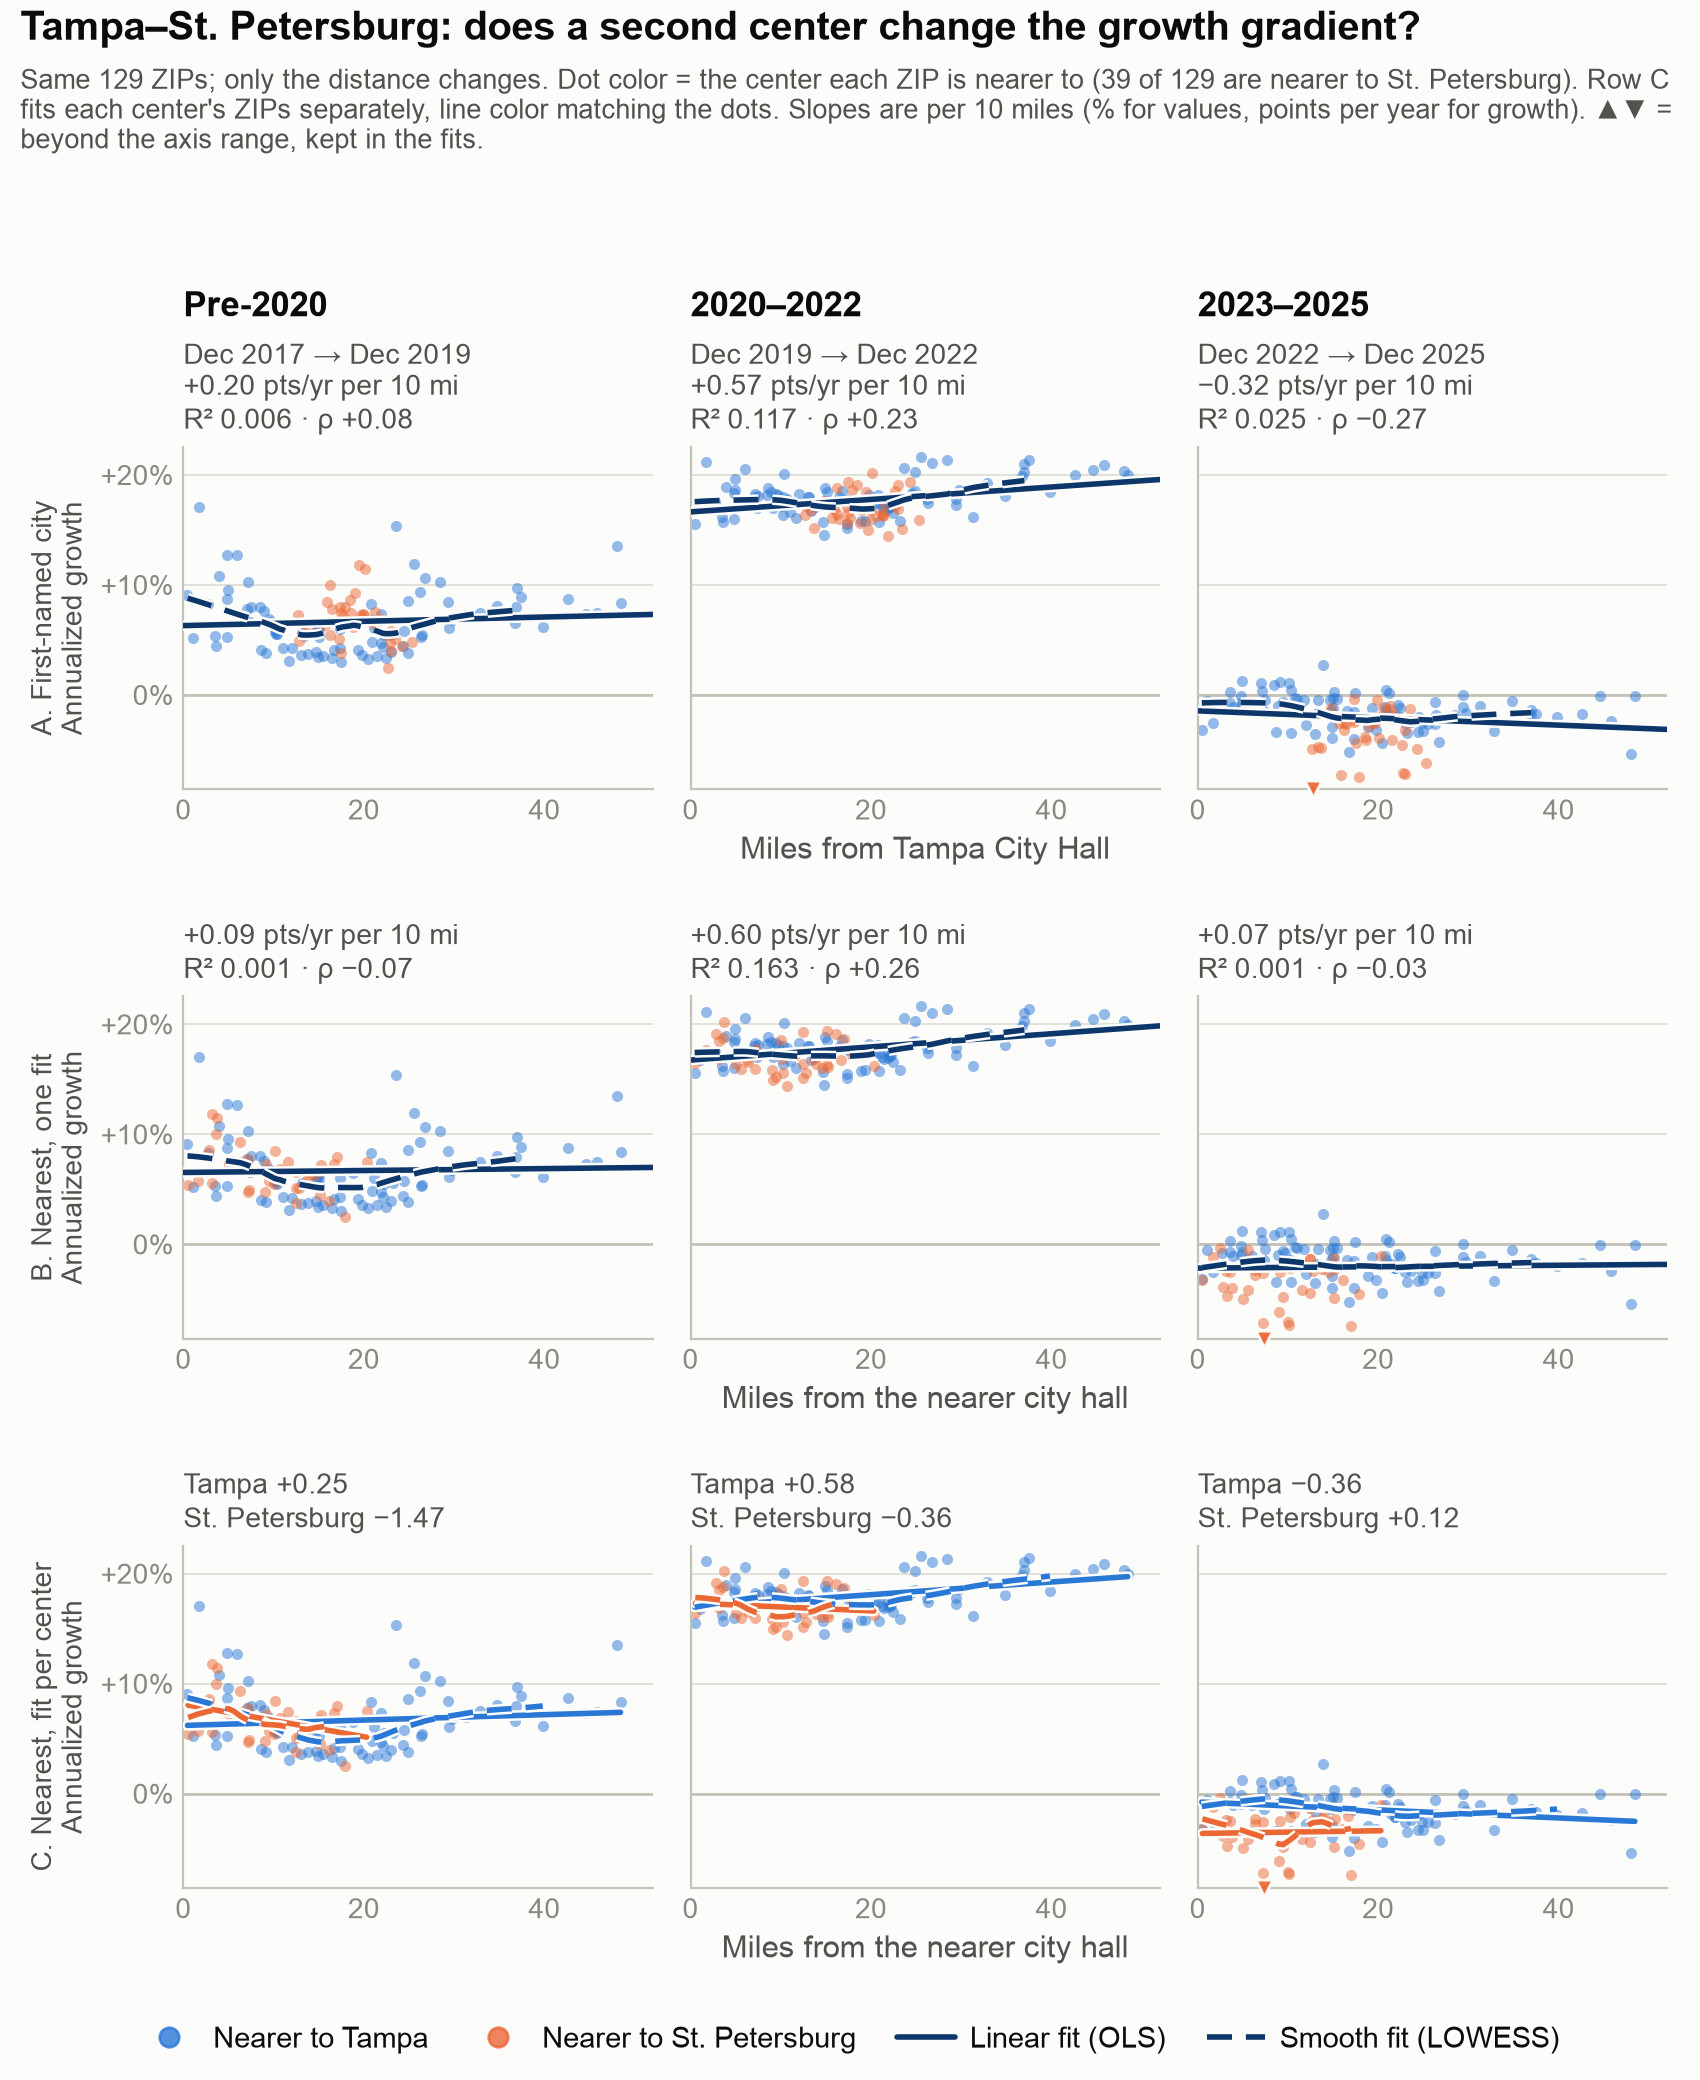
\includegraphics[width=.49\linewidth]{2_2_two_center_growth_tampa}\par\vspace{4pt}
\refstepcounter{fignum}\label{fig:twocenterTampa}
{\small\raggedright\textbf{Figure \thefignum.} Tampa-St. Petersburg level and growth fits measured from Tampa, St. Petersburg, and
the nearer city hall. The negative later slope is visible from Tampa city hall, but not with the nearer-center measure.\par
\footnotesize\textit{Sources:} Zillow Research (ZHVI) and U.S. Census Bureau geography.\par}
\end{figure}

The Tampa-St. Petersburg panels lead to the same design lesson but a different substantive pattern. Changing the center alters
both individual distances and the later-period conclusion. The slope from Tampa city hall changes sign, while the nearer-center
slope is close to zero. A stronger follow-up would use travel time to several employment centers and would test whether those
centers changed between 2019 and 2025, rather than assuming that either city hall represents every household's destination.

\clearpage
\footnotesize
\begin{thebibliography}{99}
\setlength{\itemsep}{3pt}
\setlength{\parsep}{0pt}
\bibitem{alonso1964location} W. Alonso. \textit{Location and Land Use: Toward a General Theory of Land Rent}. Harvard University
Press, 1964. \url{https://doi.org/10.4159/harvard.9780674730854}.
\bibitem{waddell1993residential} P. Waddell, B. J. L. Berry, and I. Hoch. Residential property values in a multinodal urban area:
New evidence on the implicit price of location. \textit{Journal of Real Estate Finance and Economics}, 7(2):117-141, 1993.
\url{https://doi.org/10.1007/BF01258322}.
\bibitem{mokhtarian2004telecommuting} P. L. Mokhtarian, G. O. Collantes, and C. Gertz. Telecommuting, residential location, and
commute-distance traveled. \textit{Environment and Planning A}, 36(10):1877-1897, 2004.
\url{https://doi.org/10.1068/a36218}.
\bibitem{barrero2023evolution} J. M. Barrero, N. Bloom, and S. J. Davis. The evolution of work from home. \textit{Journal of
Economic Perspectives}, 37(4):23-50, 2023. \url{https://doi.org/10.1257/jep.37.4.23}.
\bibitem{brueckner2023spatial} J. K. Brueckner, M. E. Kahn, and G. C. Lin. A new spatial hedonic equilibrium in the emerging
work-from-home economy? \textit{American Economic Journal: Applied Economics}, 15(2):285-319, 2023.
\url{https://doi.org/10.1257/app.20210190}.
\bibitem{ramani2021donut} A. Ramani and N. Bloom. The donut effect of COVID-19 on cities. NBER Working Paper 28876, 2021,
revised December 2022. \url{https://doi.org/10.3386/w28876}.
\bibitem{gupta2022flattening} A. Gupta, V. Mittal, J. Peeters, and S. Van Nieuwerburgh. Flattening the curve: Pandemic-induced
revaluation of urban real estate. \textit{Journal of Financial Economics}, 146(2):594-636, 2022.
\url{https://doi.org/10.1016/j.jfineco.2021.10.008}.
\bibitem{ahrend2023expanding} R. Ahrend et al. Expanding the doughnut? How the geography of housing demand has changed since the
rise of remote work with COVID-19. OECD Regional Development Papers 54, 2023.
\url{https://doi.org/10.1787/cf591216-en}.
\bibitem{dingel2020jobs} J. I. Dingel and B. Neiman. How many jobs can be done at home? \textit{Journal of Public Economics},
189:104235, 2020. \url{https://doi.org/10.1016/j.jpubeco.2020.104235}.
\bibitem{mondragon2022housing} J. A. Mondragon and J. Wieland. Housing demand and remote work. NBER Working Paper 30041, 2022,
revised May 2025. \url{https://doi.org/10.3386/w30041}.
\bibitem{howard2023short} G. Howard, J. Liebersohn, and A. Ozimek. The short- and long-run effects of remote work on U.S. housing
markets. \textit{Journal of Financial Economics}, 150(1):166-184, 2023.
\url{https://doi.org/10.1016/j.jfineco.2023.103705}.
\bibitem{ramani2024reshapes} A. Ramani, J. Alcedo, and N. Bloom. How working from home reshapes cities. \textit{Proceedings of the
National Academy of Sciences}, 121(45):e2408930121, 2024. \url{https://doi.org/10.1073/pnas.2408930121}.
\bibitem{fonseca2024mortgage} J. Fonseca and L. Liu. Mortgage lock-in, mobility, and labor reallocation. \textit{Journal of
Finance}, 79(6):3729-3772, 2024. \url{https://doi.org/10.1111/jofi.13398}.
\bibitem{leslie2010identification} T. F. Leslie. Identification and differentiation of urban centers in Phoenix through a
multi-criteria kernel-density approach. \textit{International Regional Science Review}, 33(2):205-235, 2010.
\url{https://doi.org/10.1177/0160017610365538}.
\bibitem{zillow2026data} Zillow Group. Housing data. Zillow Research, 2026. \url{https://www.zillow.com/research/data/}.
\bibitem{census2026acs} U.S. Census Bureau. American Community Survey 5-year data.
\url{https://www.census.gov/data/developers/data-sets/acs-5year.html}.
\bibitem{callaway2024did} B. Callaway, A. Goodman-Bacon, and P. H. C. Sant'Anna. Difference-in-differences with a continuous
treatment. NBER Working Paper 32117, 2024. \url{https://doi.org/10.3386/w32117}.
\bibitem{roberts} D. R. Roberts et al. Cross-validation strategies for data with temporal, spatial, hierarchical, or phylogenetic
structure. \textit{Ecography}, 40(8):913-929, 2017. \url{https://doi.org/10.1111/ecog.02881}.
\bibitem{rousseeuw} P. J. Rousseeuw. Silhouettes: a graphical aid to the interpretation and validation of cluster analysis.
\textit{Journal of Computational and Applied Mathematics}, 20:53-65, 1987.
\url{https://doi.org/10.1016/0377-0427(87)90125-7}.
\bibitem{breiman2} L. Breiman. Random forests. \textit{Machine Learning}, 45(1):5-32, 2001.
\url{https://doi.org/10.1023/A:1010933404324}.
\bibitem{sklearn} F. Pedregosa et al. Scikit-learn: machine learning in Python. \textit{Journal of Machine Learning Research},
12:2825-2830, 2011. \url{https://jmlr.org/papers/v12/pedregosa11a.html}.
\end{thebibliography}

\end{document}
